\documentclass{article}

% \usepackage{standalone}
 \usepackage{graphicx}
% \usepackage{media9}
%\graphicspath{{./images/}}
% \usepackage{amsmath}
\usepackage{multicol}
\usepackage{hyperref}
% \usepackage{setspace}                       \usepackage{geometry}          
%  \usepackage{longtable}                      
% \usepackage{chicago}                  
% \usepackage{times} 
% \usepackage{paracol}   % parallel columns    
% \usepackage[dvipsnames]{xcolor}       \usepackage{calc}                                      

% \usepackage{tikz}
% \usetikzlibrary{positioning, shadows, arrows, automata, shapes, calc, decorations.pathreplacing,calligraphy}

\title{Notes on Experiments}
\author{KLMW}
\begin{document}
\maketitle
\tableofcontents \newpage
\section{Notes on Experiments}
This is a record of experiments testing the effect of varying parameters. The tests are grouped in two parts: tests of the base model of city and the production sector, and tests of the housing market parameters. 

In the first part the goal is to ensure that the platform underlying the housing market behaves as expected. One important policy result was found: Transportation costs, which are under the control of local governments, have a very large effect.

In the second part we find that the proportion of owneroccupiers is sensitive to  several policy instruments. 

Complex combinations of policies are computationally intensive and are not explored in this section.

\vspace{.5cm}

{\tiny
BASELINE PARAMETERS: Initial values most commonly used 
\begin{verbatim}

        # LABOUR MARKET AND FIRM PARAMETERS
            'subsistence_wage': 40000., # RURAL WAGE,  psi, 
            'init_city_extent': 10.,    # 
            'seed_population': 400,     # POPULATION AT CENTRE
            'init_wage_premium_ratio': 0.2, # WAGE PREMIUM AS FRACTION OF SUBSISTENCE WAGE

            # PARAMETERS MOST LIKELY TO AFFECT SCALE
            'c': 300                    # TRANSPORT COST PER UNIT DISTANCE
            'price_of_output': 10,      # WORLD PRICE FOR FIRM
            'density':600,              # WORKERS PER BLOCK  
            'A': 3000,                  # SCALE FACTOR 
            'alpha': 0.18,              # EXPONENT ON FIRM CAPITAL
            'beta':  0.75,              # EXPONENT ON FIRM LABOUR
            'gamma': 0.12,              # EXPONENT ON AGGLOMERATION POPULATION
            'overhead': 0.5,            # FIRM OVERHEAD COST AS WAGE FRACTION
            'mult': 1.2,                # AGGLOM POP IS MULT for x N
            'adjN': 0.15,               # ADJUSTMENT RATE WORKER COUNT
            'adjk': 0.10,               # ADJUSTMENT RATE FIRM CAPITAL
            'adjn': 0.15,               # ADJUSTMENT RATE FIRM WORKFORCE
            'adjF': 0.02,               # ADJUSTMENT RATE NO OF FIRMS
            'adjw': 0.05,               # ADJUSTMENT RATE WAGE
            'dist': 1,                  # DISTANCE FROM CENTER
            'init_F': 100.0,            # INITIAL NUMBER OF FIRMS
            'init_k': 500.0,            # INITIAL CAPITAL STOCK OF FIRMS
            'init_n': 100.0,            # INITIAL LABOURFORCE OF FIRMS

            # HOUSING AND MORTGAGE MARKET PARAMETERS
            'mortgage_period': 5.0,       # T, YEARS TO RENEGOTIATION OF MORGAGE
            'working_periods': 40,        # YEARS IN THE WORKFORCE
            'savings_rate': 0.3,          # FRACTION SAVED OUT OF WAGE PLUS RENT
            'discount_rate': 0.07,        # 1/delta    Check THIS
            'r_prime': 0.05,              # BANK RATE          
            'r_margin': 0.01,             # BANK PROFIT          
            'property_tax_rate': 0.04,    # tau,  ANNUAL PROPERTY TAX RATE
            'housing_services_share': 0.3,# a, OF SUBSISTENCE WAGE
            'maintenance_share': 0.2,     # b. OF HOUSING SERVICES
            'max_mortgage_share': 0.9,    # OF SALE PRICE
            'ability_to_carry_mortgage': 0.28,# MAX SHARE OF INCOME  FOR MORTGAGE PAYMENTS
            'wealth_sensitivity': 0.1,    # OF INTEREST CHARGE 
            'capital_gains_tax_person': 0.0,  # 0-1 SHARE F CAPITAL GAIN
            'capital_gains_tax_investor': 1,  # 0-1 SHARE F CAPITAL GAIN
    
\end{verbatim}
}
\newpage

% \subsection{parameters}
% \begin{verbatim}

% \end{verbatim}

\section{Base model of city and the production sector}
\newpage
 \subsection{The price. of output}
Underlying the housing analysis is an economic model of the city including firms and transportation.  The first question for an economist is likely to be is, ``Does the system respond to an increase in demand for its export product in the expected ways?'' The following figure shows that it does. 


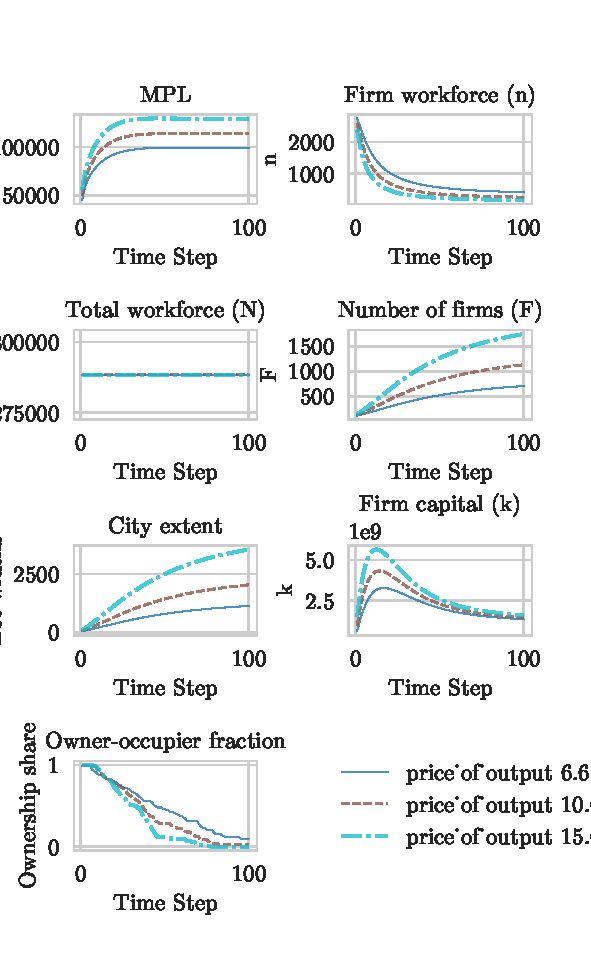
\includegraphics[scale=1]{fig/Analysis/price3.pdf}

\newpage %%%%%%%%%%%%%%%%%%%%%%%%%%%%%%%%%%
\subsection{Capital gains taxes for investors}
In our model capital gains provide a motive for the purchase of existing housing. If investors enter the market for existing owner-occupiers, we would expect that they would bid up the price of housing and squeeze out owner-occupiers. We see this effect in the lower left of the following figure. This is occurring in a model with a perfectly elastic housing supply at the city edge. Notice there is no effect on the paths of labour or other vars.
\begin{figure}
    \centering
    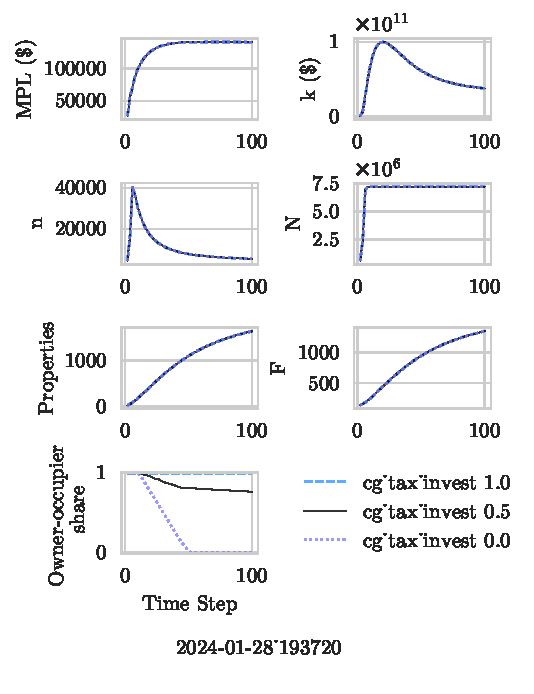
\includegraphics{fig/Analysis/cg_tax_invest-[1- 0.5-0.0]_193720.pdf}
    \caption{Varying the capital gains tax on investors}
    \label{fig:enter-label}
\end{figure}

There is a range of rates between 0.5 and 0 capital gains tax over which the ownership share responds just as it does to 0.5 -  staying at 80\%. If we set the rate for investors to say 35\% and vary the rate for homeowners we find that the decisive factor in shifting ownership is that the capital gains tax rate for investors is lower than the rate for homeowners.  Real tax systems are more complicated than they are in our model - various conditions affect the ``effective tax rate''. Since capital gains on one's principal residence are not taxed, the tax treatment of capital gains on investment properties is potentially significant. Only 50\% of total capital gains are ] taxable, essentially reducing the marginal income-tax rate for these gains by half for investors. Capital gains can be sheltered in numerous other ways as well under the tax rules, but we are not expert in tax law and do not know the extent to which capital gains on investment properties might be sheltered enough to affect ownership patterns. The effect is dramatic in our model and further study.% %REITs buy and hold property that's too expensive for most investors to purchase individually, putting residential investment property within reach of many more people. 

\begin{figure}
    \centering
  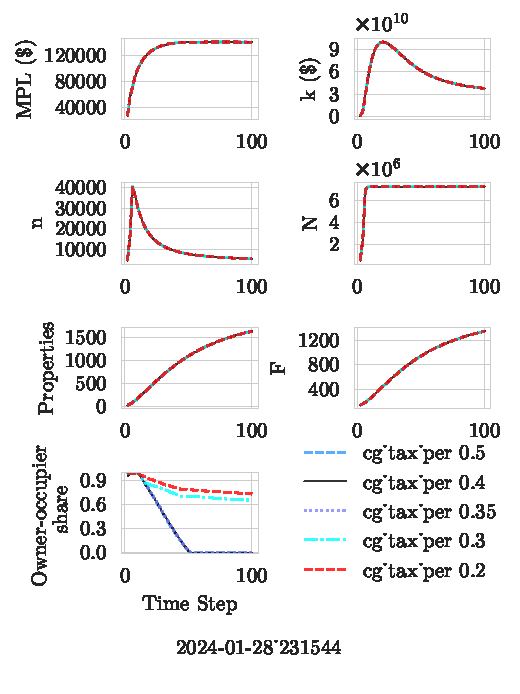
\includegraphics{fig/Analysis/cg_tax_per-2024-01-28_231544}
    \caption{Varying the capital gains tax on owner occupiers}
    \label{fig:enter-label}
\end{figure}



 \subsection{Change Density}
 This experiment verifies that the labour-market/urban model that is the platform for the housing market analysis behaves exactly as expected when density increases. mpl, n, N, F, E, and k all rise. 

 We also see overshoot in the firm workforce that is a result of a low partial adjustment rate.

 

 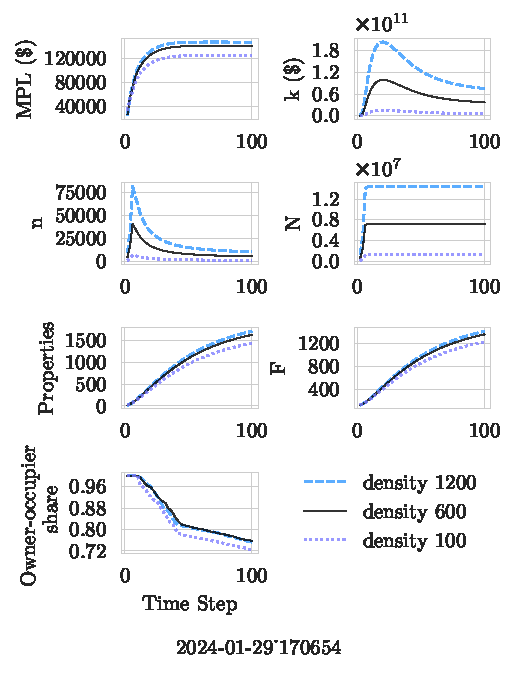
\includegraphics[]{fig/Analysis/density-2024-01-29_170654.pdf}


\newpage %%%%%%%%%%%%%%%%%%%%%%%%%%%%%%%%%%
\subsection{Wage  adjustment  speed} 
In our ABM, firms use information about the  marginal productivity of labour and capital to set targets for the current period, then adjust the number or workers and capital stock toward the target. The dynamic behaviour of the labour and capital are sensitive to the adjustment rates. 

Overshoot in the firm workforce, $n$, at low adjustment rates persists. It is interesting to not that with more rapid adjustment,  firm workforce is higher, firm capital stock. is higher and the number of firms is lower. If firms adjust labour more quickly they grow more rapidly sucking  up the labour supply before the number of firms can expand. 

Surprisingly, overshoot in capital declines as the rate of adjustment in the wage increases. The explanation is probably simply that when labour approaches  the profit maximizing level more quickly, the agent makes better decisions about the capital stock



 \includegraphics[]{fig/Analysis/adjw-2024-01-30_002252.pdf}

 \begin{figure}
     \centering
     \includegraphics[width=0.5\linewidth]{adjw-2024-01-30_002252.pdf}
     \caption{Enter Caption}
     \label{fig:enter-label}
 \end{figure}


 
\newpage %%%%%%%%%%%%%%%%%%%%%%%%%%%%%%%%%%
\subsection{Rate at which firms enter}
If  the number of firms is constant,  any increase in city size results in inreases in the number of workers in a firm. We allow firm entry. we assume that potential entrants (start-up entrepreneurs) observe growth in some variables and interpret it as an opportunity. We use wage growth, but several others would do as well. The rate of entry then affects the size of firms - more firm entry leads to lower efirm sizes.

 
\newpage %%%%%%%%%%%%%%%%%%%%%%%%%%%%%%%%%%
\subsection{Capital gains taxes for investors}

\newpage %%%%%%%%%%%%%%%%%%%%%%%%%%%%%%%%%%

\subsection{High Gamma}
Very high levels of the agglomeration parameter Gamma are implausible. They drive up marginal productivity, causing very rapid growth, drive down firm size because the first worker is extremely productive but the MPL falls rapidly. Very small firms with high levels of capital multiply. Rapidly rising prices encourage investors while savings-limited owner-occupiers are squeezed out.

Higher agglomeration effects make land rents higher and increase the gains to investors, resulting in more rapid financialization of the housing stock.

%   we can check
 
% \begin{tabular}{|c|c||c|c||c|c|}
% mpl  & up   & n   & up & N   &  up \\
% F    & up   & E   &  up  &  k & up
% \end{tabular} 

 \hspace*{-2.5cm}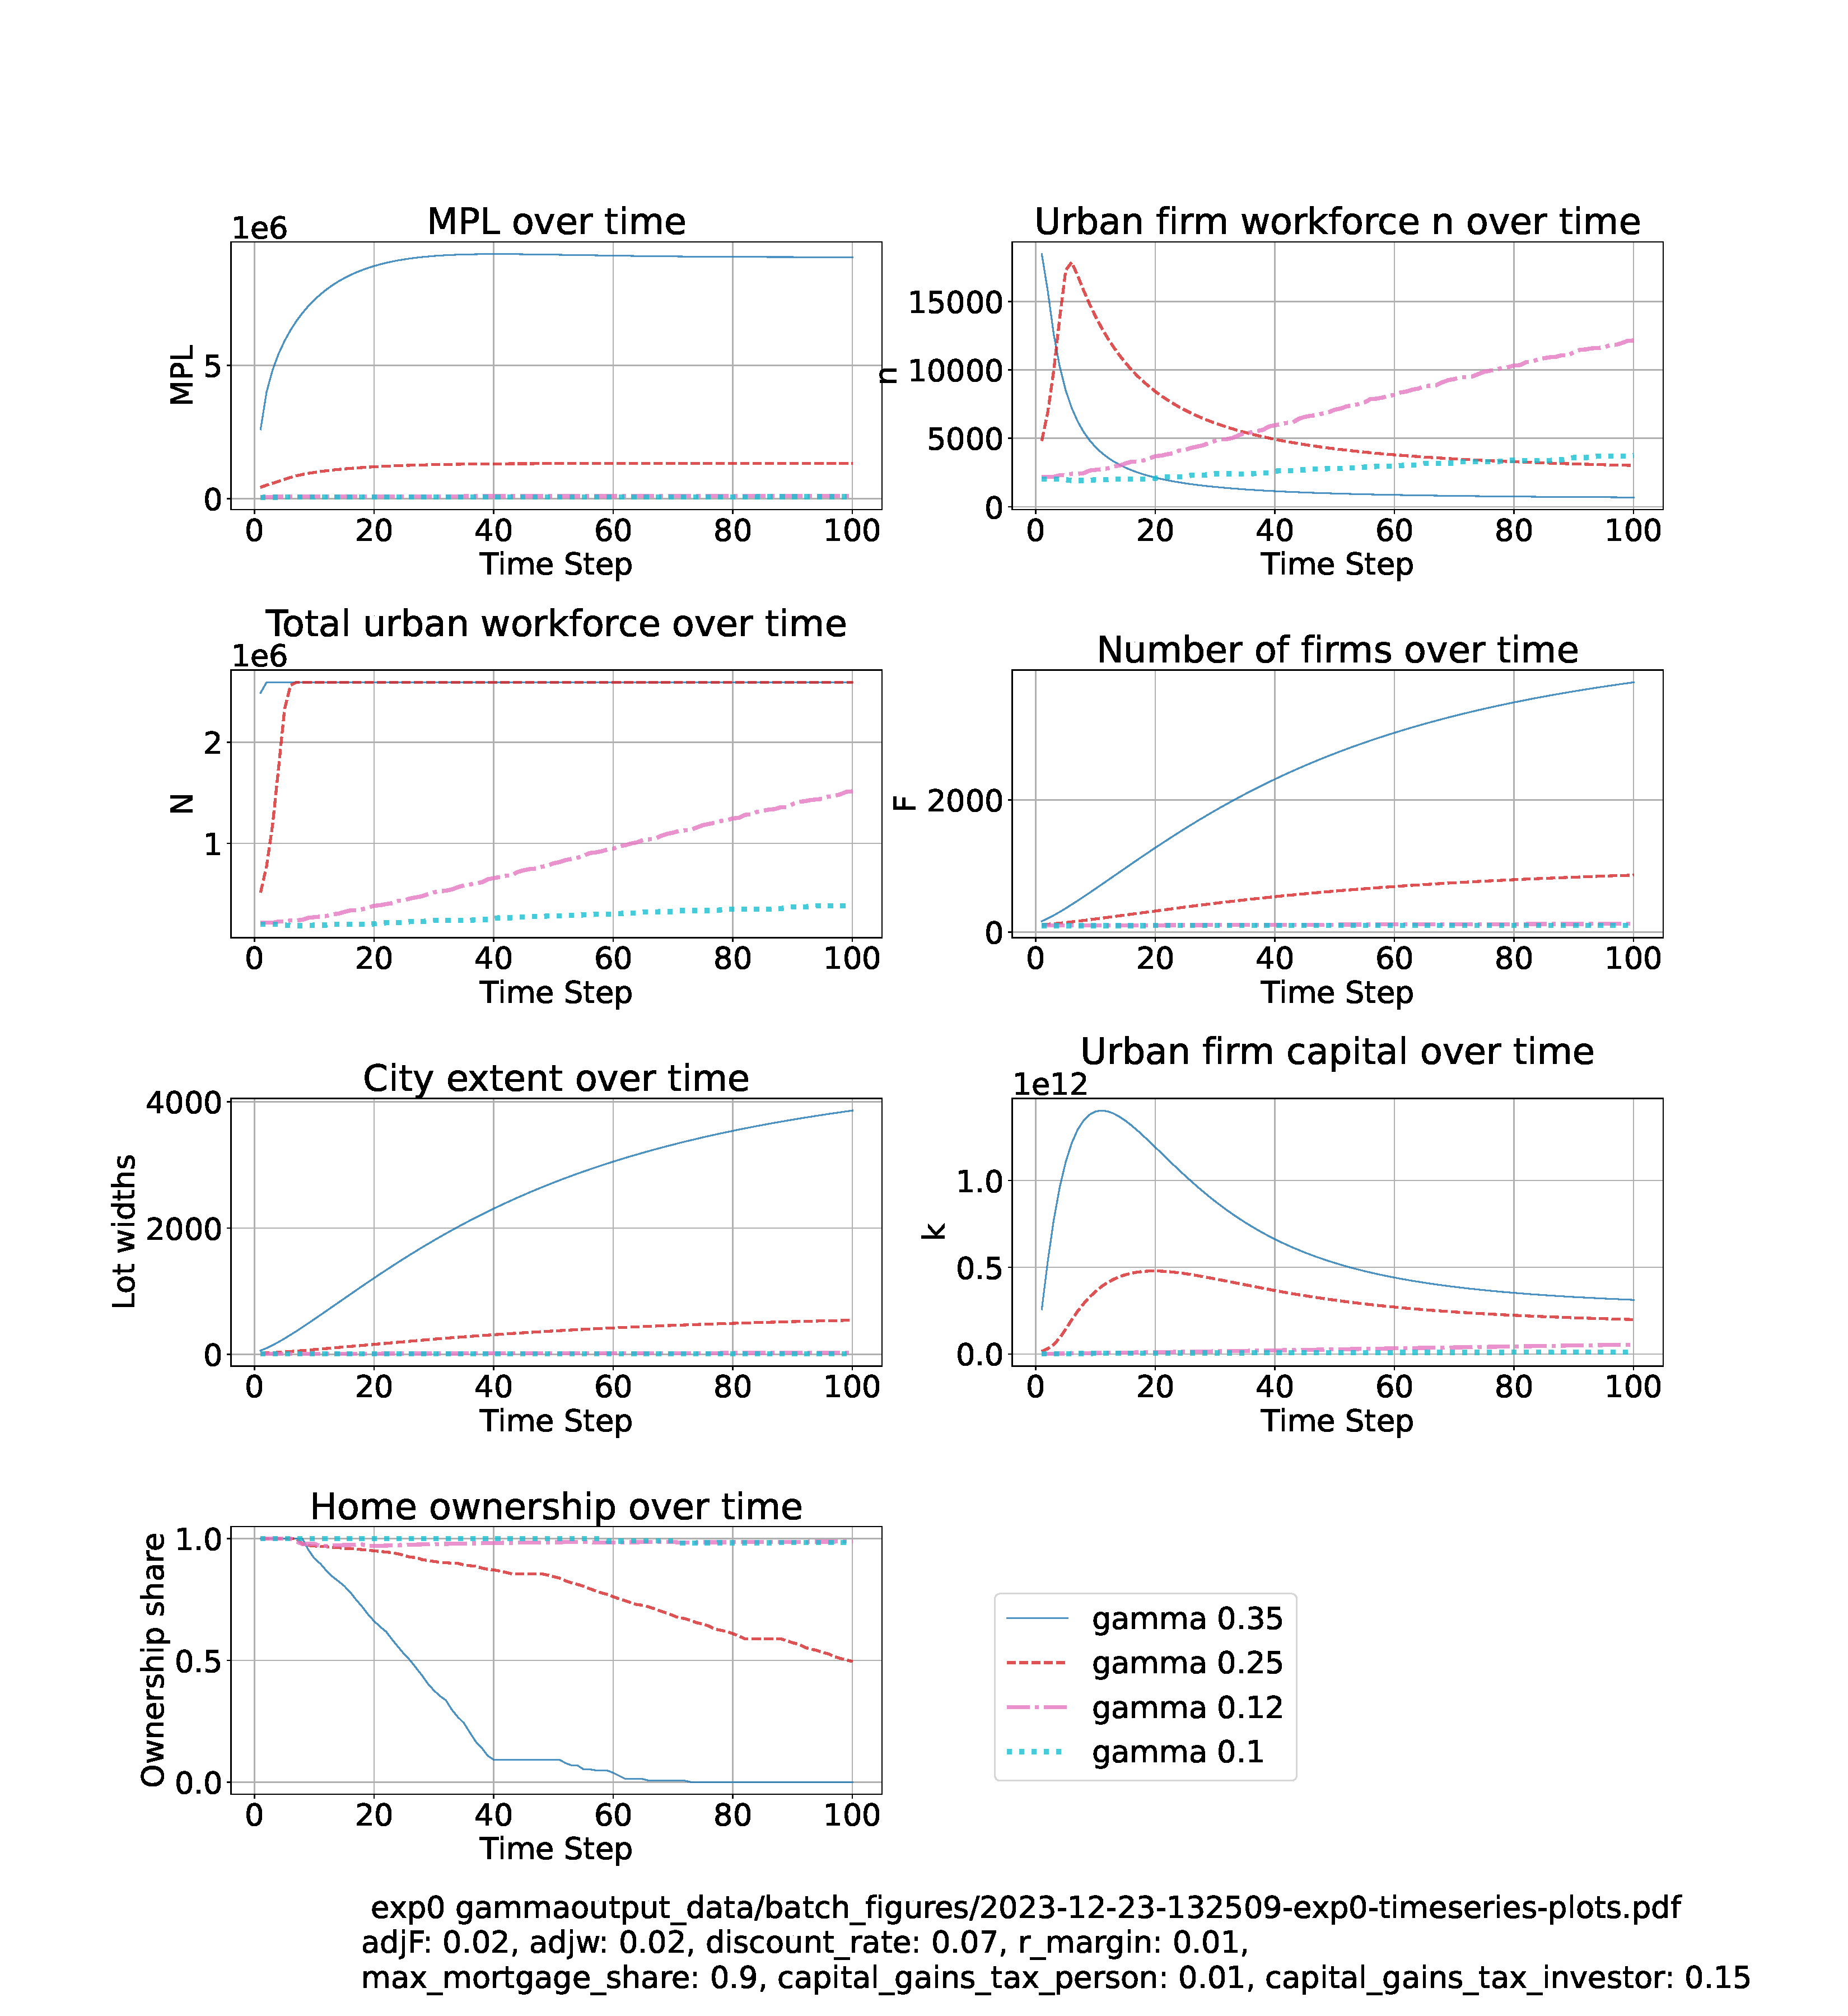
\includegraphics[trim= 1.5cm 3.65cm 2cm 4.0cm, clip, scale=.28]{fig/Analysis/Gamma-5-30.pdf}

\newpage %%%%%%%%%%%%%%%%%%%%%%%%%%%%%%%%%%

\subsection{Low Gamma}
Low levels of the agglomeration parameter Gamma are plausible but city growth requires a level high enough to overcome decreasing returns in production.

At near-zero levels population is hiring at the firm level sharply affects  the marginal product and randomization in saving the share of housing that is owner occupied.
 
% \begin{tabular}{|c|c||c|c||c|c|}
% mpl  & up   & n   & up & N   &  up \\
% F    & up   & E   &  up  &  k & up
% \end{tabular} 

 \hspace*{-2.5cm}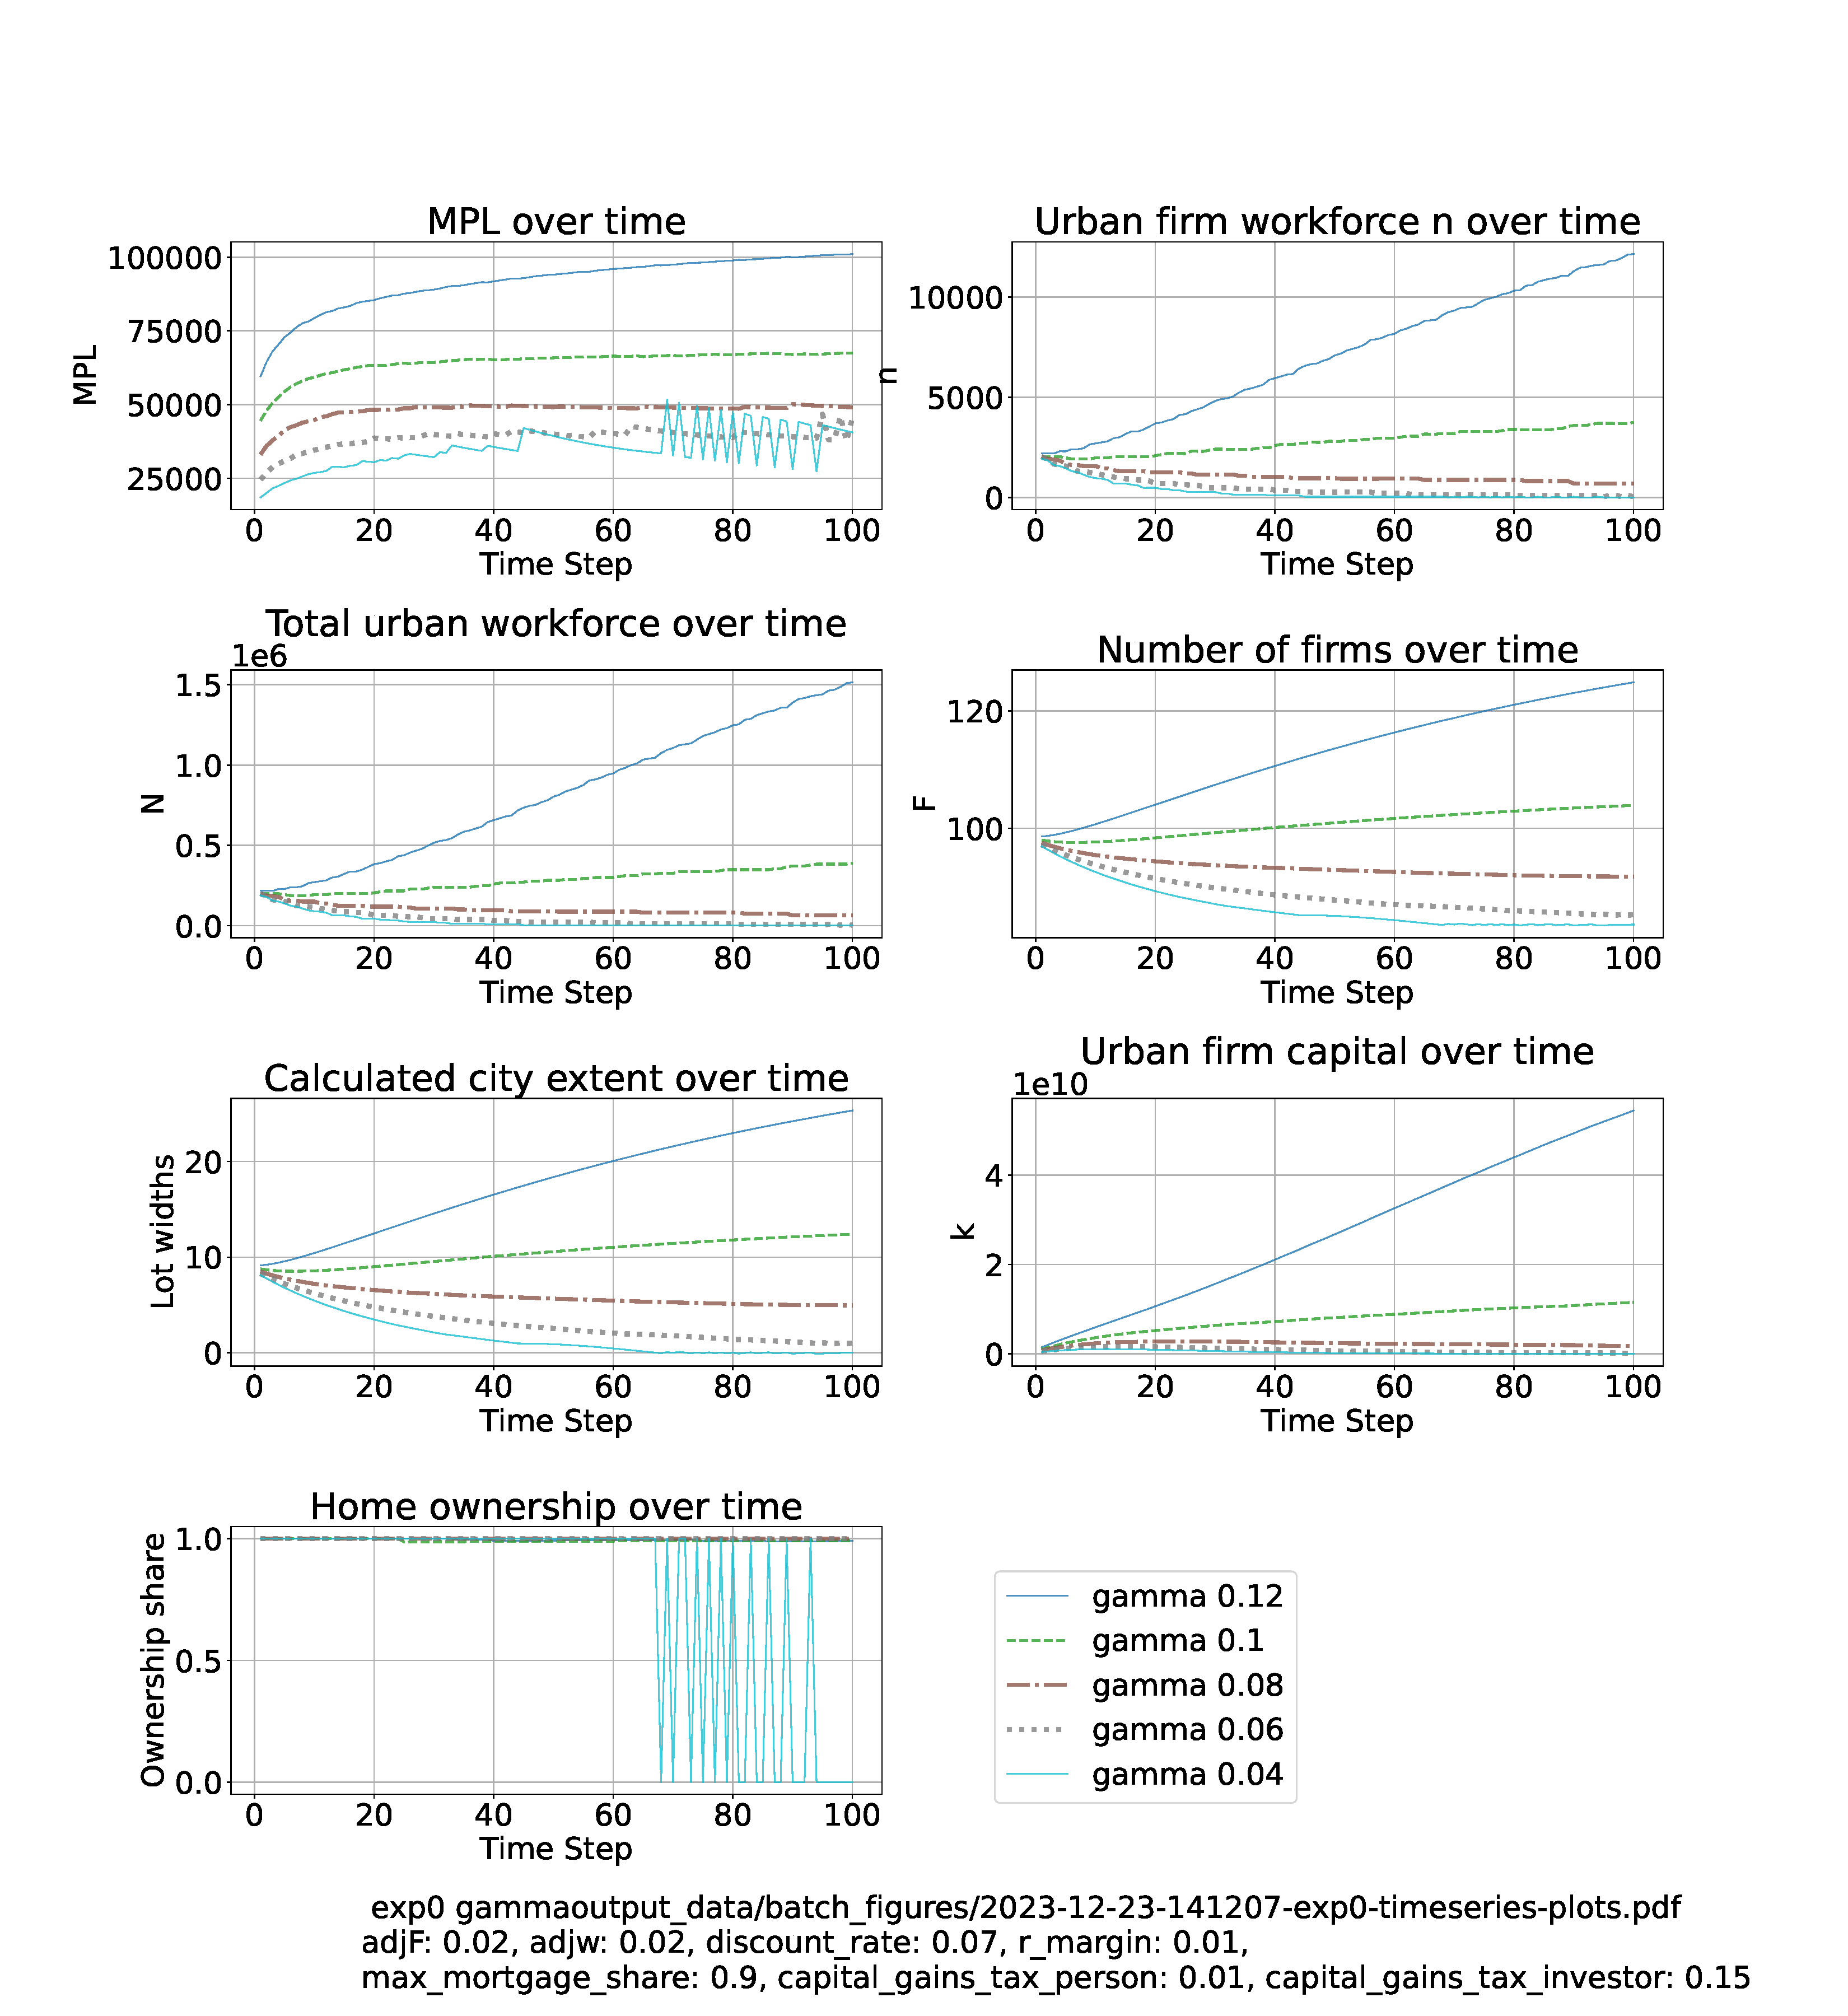
\includegraphics[trim= 1.5cm 3.65cm 2cm 4.0cm, clip, scale=.3]{fig/Analysis/Gamma-low-5-30.pdf}

\newpage %%%%%%%%%%%%%%%%%%%%%%%%%%%%%%%%%%

\subsection{Change adjF - the growth rate of number of firms }

\begin{multicols}{2}
\begin{tabular}{c|c}
  mpl   &  up\\
  n   &  dn\\
  N   &  up\\
  F   & up \\
  E   &  up\\
  k   & dn
\end{tabular}

  notice the way firm number and size reverse as the adjustment speed changes. This makes sense
  
\end{multicols}

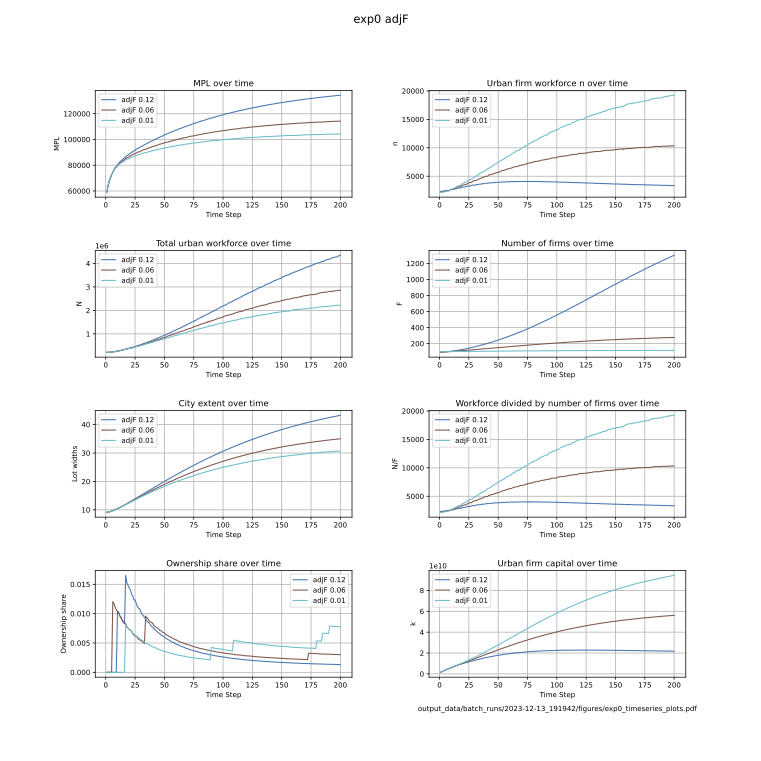
\includegraphics[scale=.55]{fig/Analysis/AdjF.png}

Notice too how MPL  is higher with a more rapid firm size adjustment. It keeps  firm workforce size down and pushes up MPL down, 

  Interestingly, city size is larger with faster growth of firm numbers. this is likely because with more firms hiring the population of the city grows faster.

  Ownership bounces around due to randomization of savings.


TO DO RE RUN WITH CURRENT PARAMETERS AND GRAPHING
%%%%%%%%%%%%%%%%%%%%%%%%%%%%%%%%%%%%%%%%%%%%%
\newpage
% \subsection{parameters}
% \begin{verbatim}

% \end{verbatim}

 \subsection{x12-15 010050, Change  Both adjF and adjn}

 REDO AS 2x2
\begin{multicols}{2}
\begin{tabular}{c|c}
  mpl  &  \\
  n   &  \\
  N   &  \\
  F   &  \\
  E   &  \\
  k   & 
\end{tabular} 
Only three cases show (gold, turquoise, and purple). firm size and number show the same patterns as when just adF is changed 
\end{multicols}
% \begin{tabular}{l|c||c|c}
% parameters&&impact&\\ \hline
% & &  mpl  &  \\
% & &    n   &  \\
% & &    N   &  \\
% & & F   &  \\ 
% & &    Extent   &  \\
% & &    k   & 
% \end{tabular} 

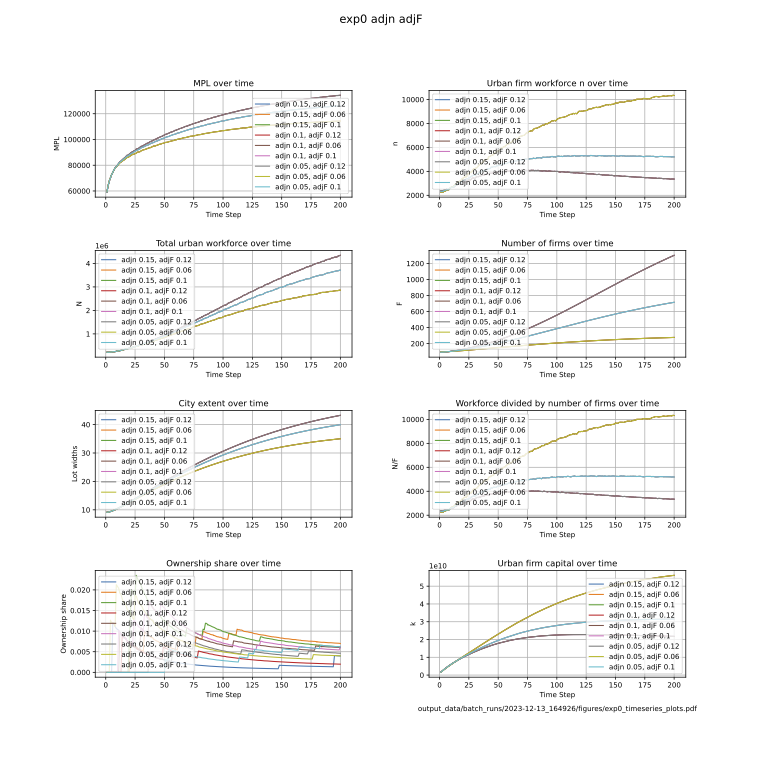
\includegraphics[scale=.55]{fig/Analysis/F-n-adjustment-speed.png}

% Subsistance wage typical 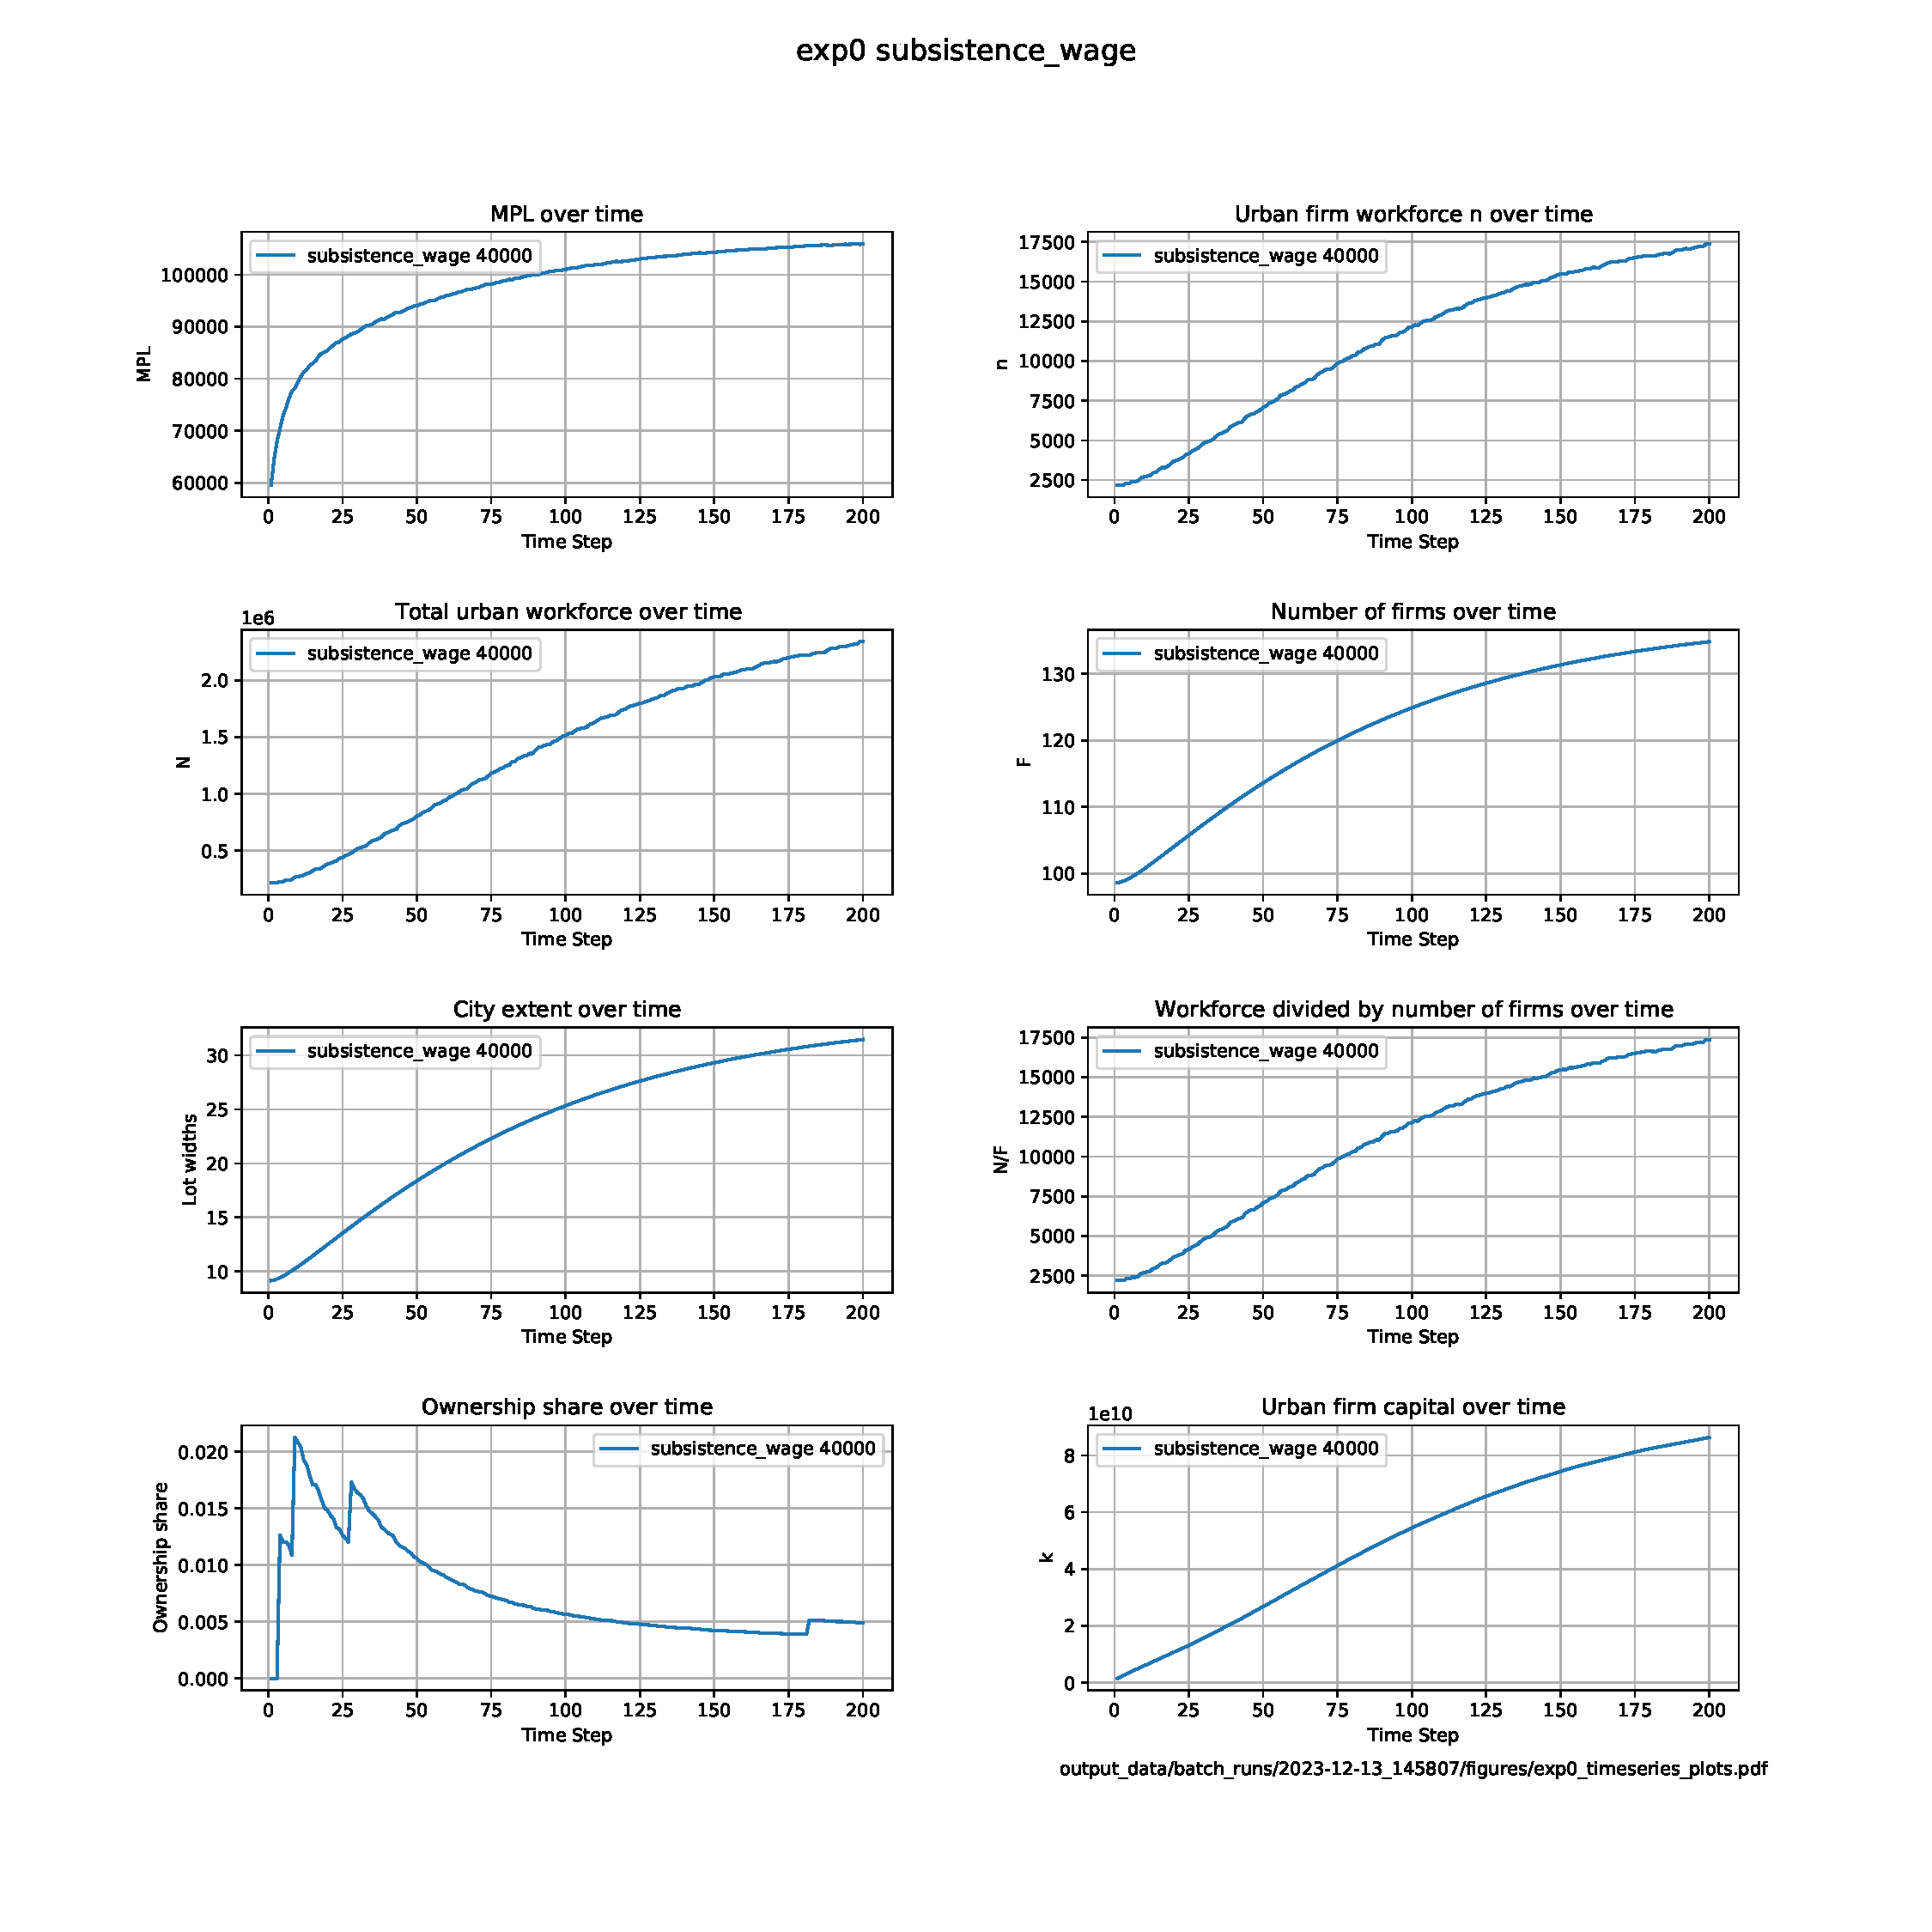
\includegraphics[scale=.55]{fig/Analysis/exp0-timeseries-plots.pdf}


We will want something like this perhaps in an early chapter. this case may not be interesting.
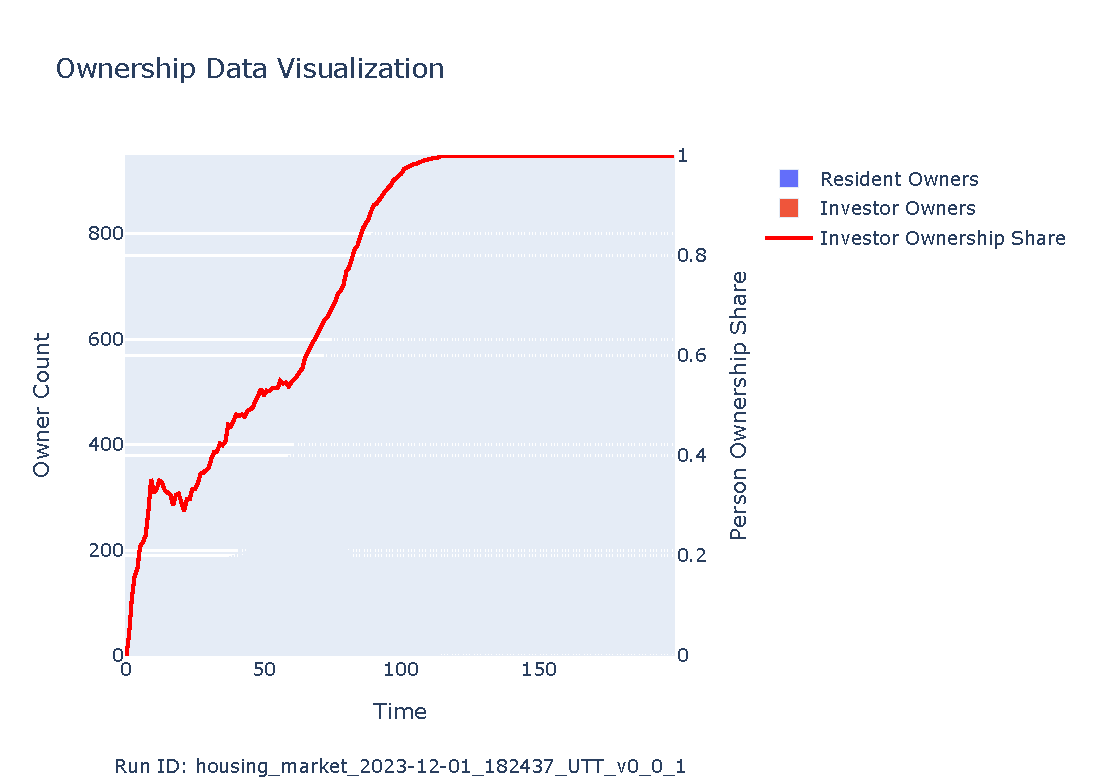
\includegraphics[scale=.95]{fig/Analysis/Ownership_Data_1.pdf}
% \subsection{parameters}
% \begin{verbatim}

% \end{verbatim}
\newpage
% \subsection{parameters}
% \begin{verbatim}

% \end{verbatim}


\newpage %%%%%%%%%%%%%%%%%%%%%%%%%%%%%%%%%%

\subsection{Alpha}
Low levels of capital productivity lead to urban decline. City growth requires a level high enough to overcome decreasing returns in production. 

We do not know why ownership drops suddenly for the very low value of alpha. It happens around the time firm capital peaks

Capital augmenting public expenditures would support growth.
 
% \begin{tabular}{|c|c||c|c||c|c|}
% mpl  & up   & n   & \textbf{down} & N   &  up \\
% F    & up   & E   &  up  &  k & up
% \end{tabular} 

 \hspace*{-2.5cm}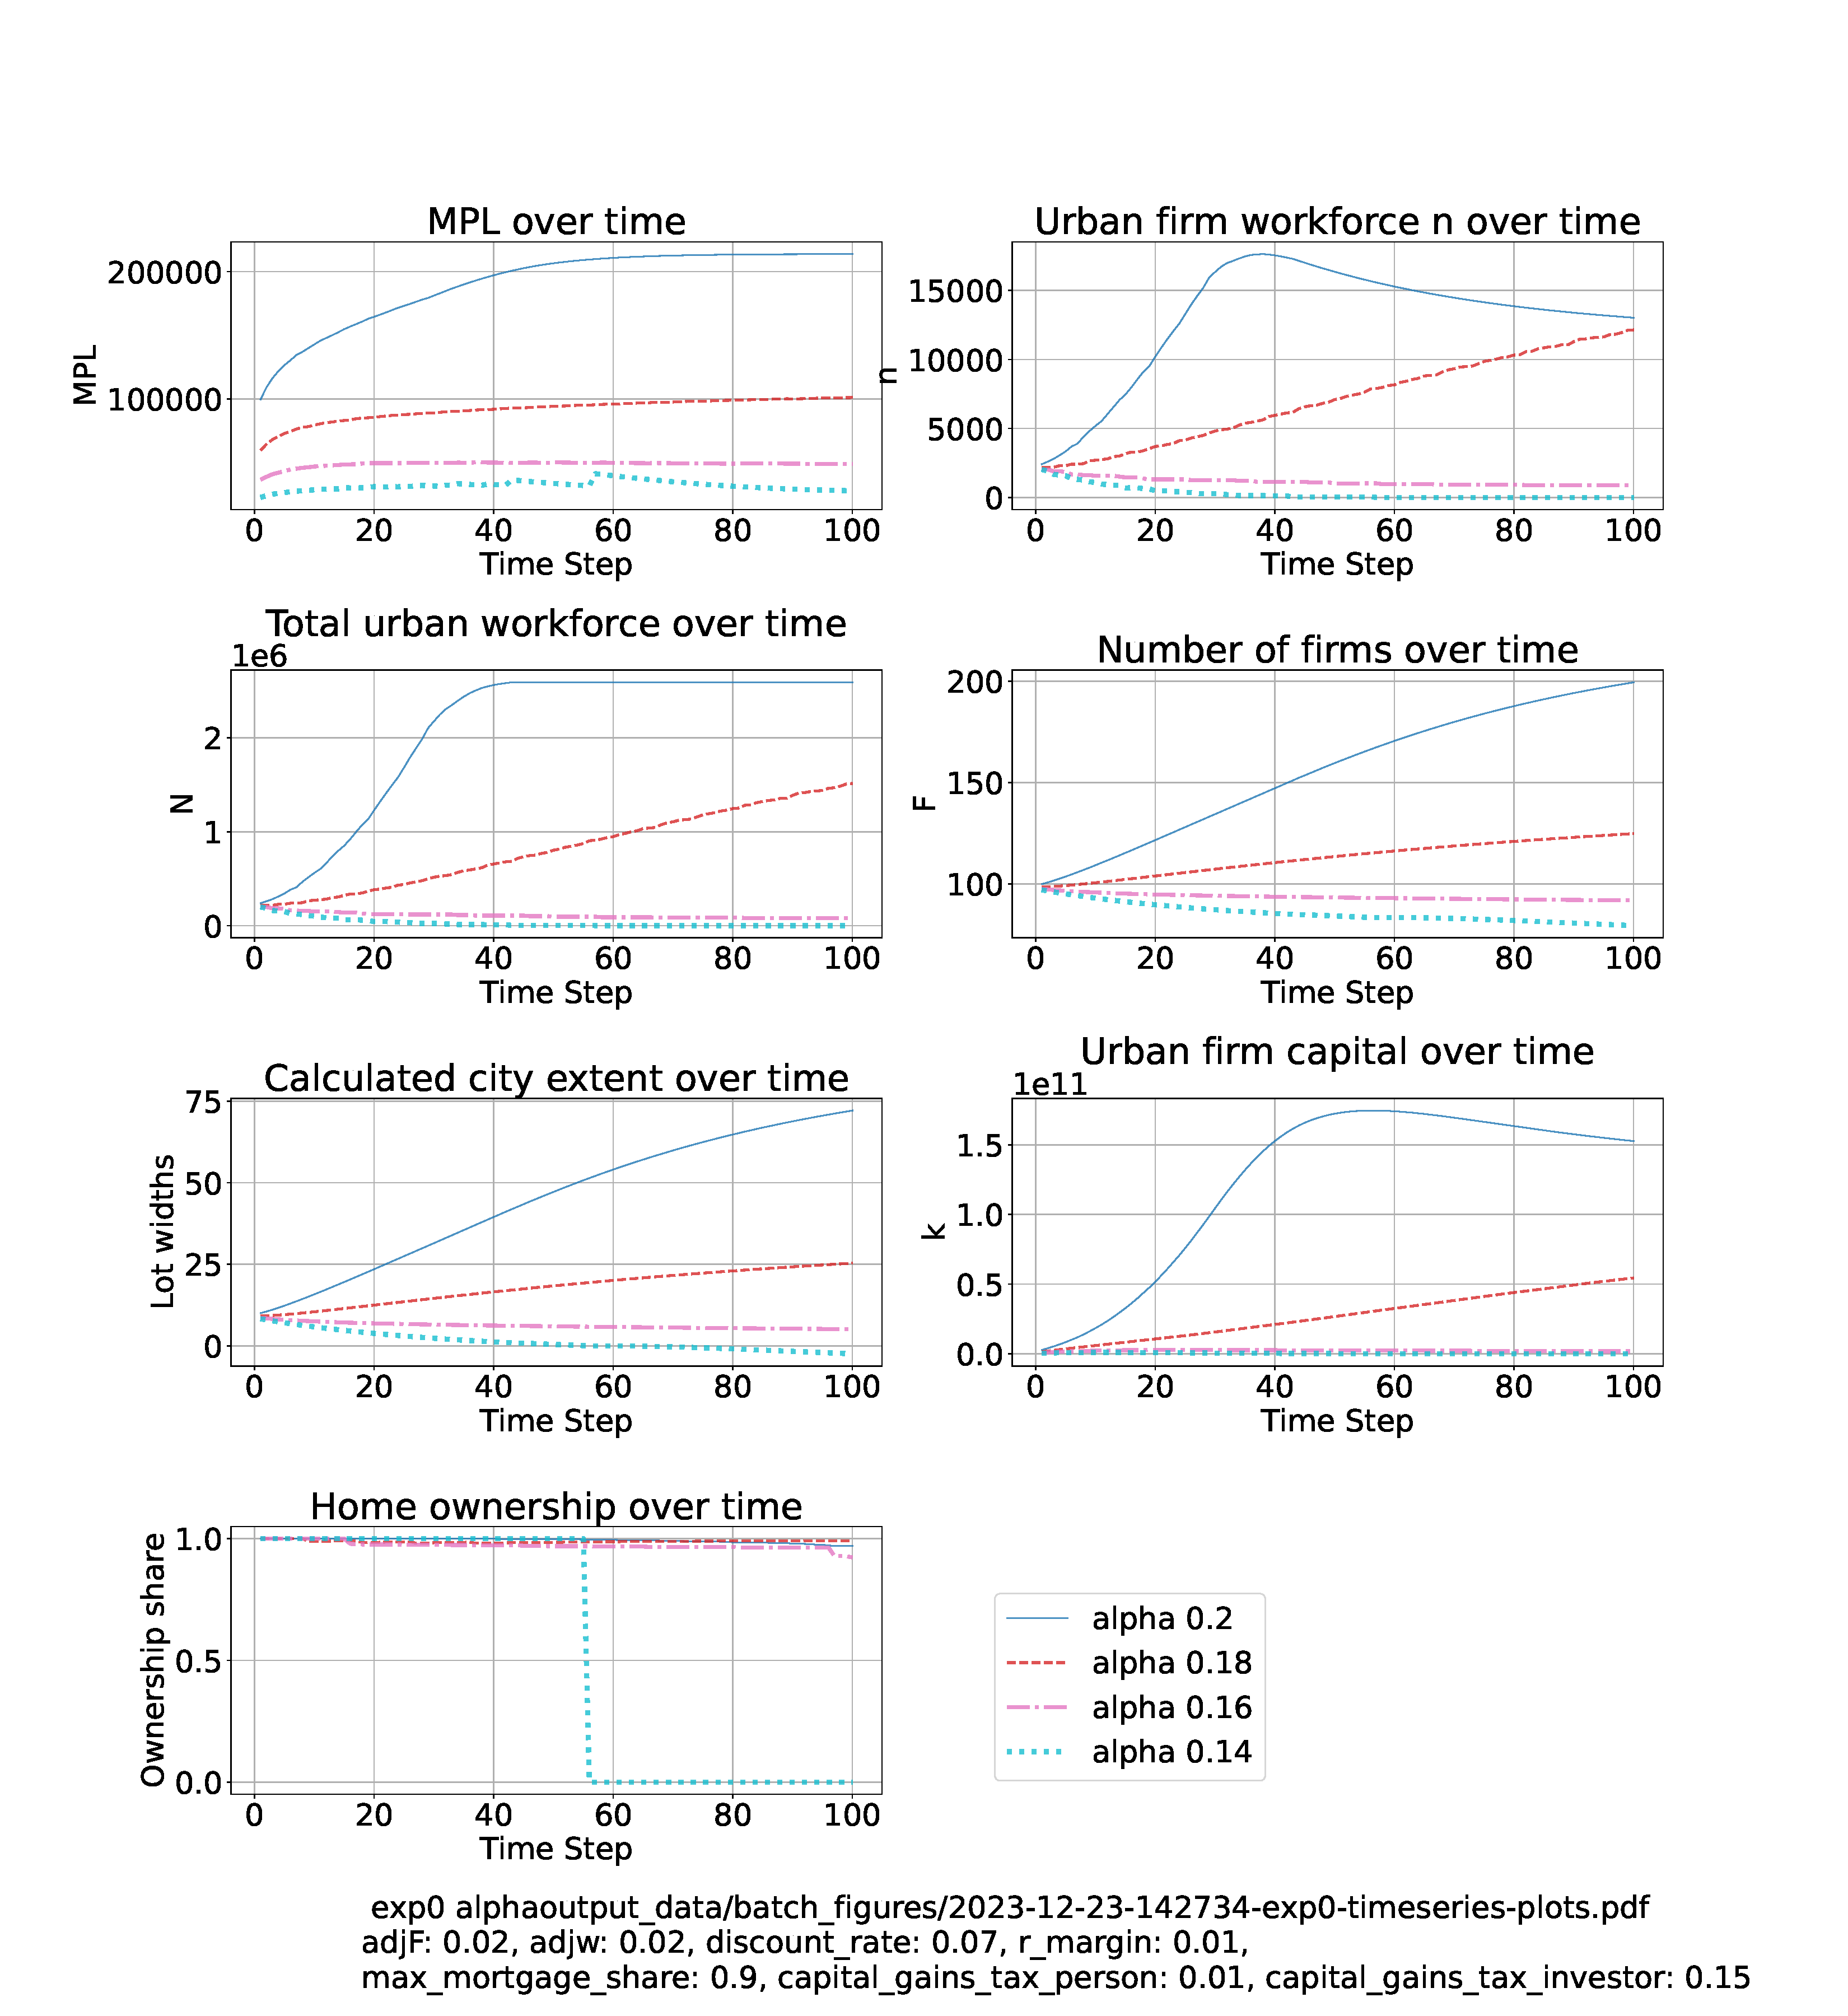
\includegraphics[trim= 1.5cm 3.65cm 2cm 4.0cm, clip, scale=.3]{fig/Analysis/Alpha-4-30.pdf}

\newpage %%%%%%%%%%%%%%%%%%%%%%%%%%%%%%%%%%

\subsection{Transportation cost c}
Transport cost affects the city extent, in turn affecting workforce size and the wealth generated on the city's land. All variables respond as expected. 
 
\begin{tabular}{|c|c||c|c||c|c|}
mpl  & null   & n   & null & N   &  null \\
F    & null   & E   &  null  &  k & null
\end{tabular} 

 \hspace{-2.5cm}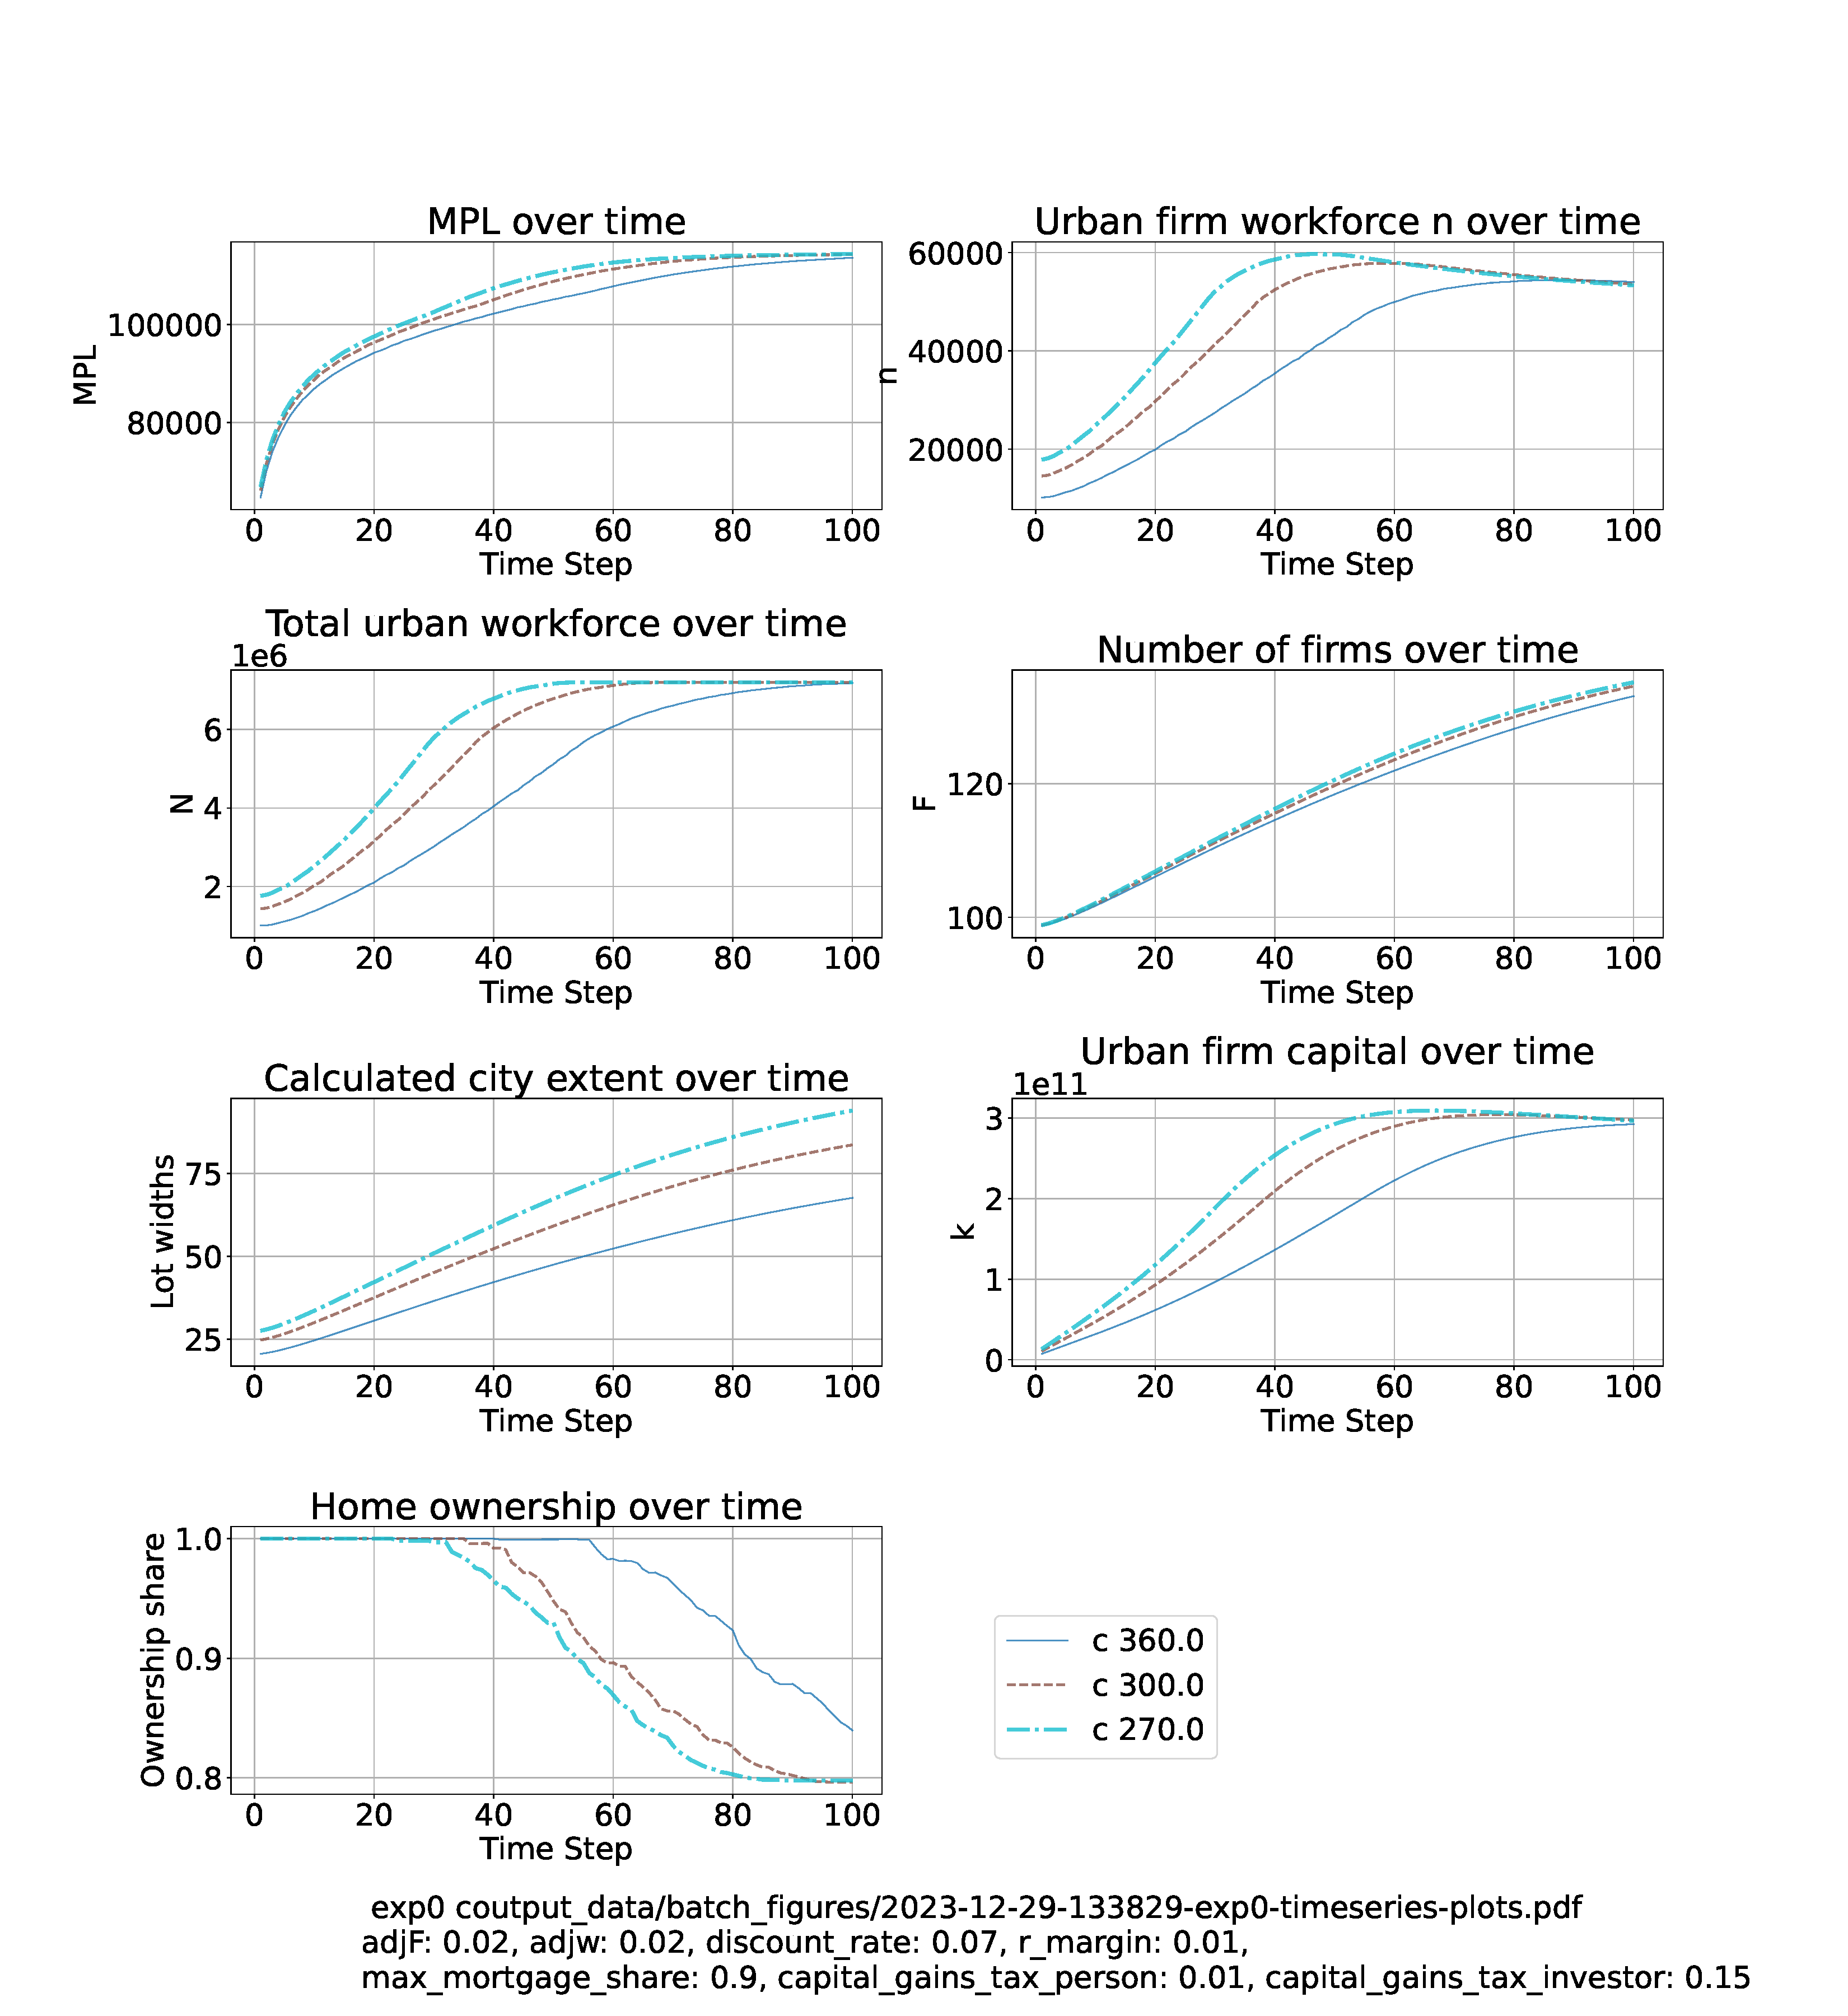
\includegraphics[trim= 1.5cm 3.65cm 2cm 4.0cm, clip, scale=.28]{fig/Analysis/Changing_Transport-cost2.pdf}

Transport cost affects both the total workforce and the total locational rents generated by a city. The response of the workforce is inversely proportional to the square of the transport cost.  

The figure above illustrates 10\% above and below our baseline value.  Reducing transport cost by 10\% increases population and total locational rents 10 \[\frac{1}{0.9 \times 0.9}=1.234568\]
the base value. This calculation assumes that wage and density do not respond as well but that the city extent does adjust.

\[Workforce\propto density * \pi \frac{\omega^2}{c^2}\]
\[Locational\ rents\propto density * \pi \frac{\omega^3}{c^2}\]\

\textbf{These relationships make transport costs the most influential single variable controlled by local authorities.} Transport systems, however, are costly in terms of land use and externalities generated or forgone.

The impact on housing ownership is curious. Home-ownership declines to about 



\newpage %%%%%%%%%%%%%%%%%%%%%%%%%%%%%%%%%%
\section{Housing sector parameters}

\subsection{Capital Gains Taxation}



Capital Gains taxes regulate the amount of future rents that owners capture.  In our model, with two classes of owners, the relative levels of capital gains taxes shift the advantage between owner-occupiers and investors, so we expect variations to affect the ownership share.


Absolute levels of capital gains taxes shift the productivity of the city from the private to the public sector. \textbf{In the current version the tax  revenues are not allocated.  In practice capital gains are a form of income and the revenues from income taxes all  go the the Federal and Provincial governments. They are not fed back into the urban economy. Since they arise form the urban process, policy makers should consider returning them to the Urban system.} 

 The following figure illustrates such a transition over a very small shift in capital gains tax for owners while holding the tax for investors constant at 15\%.

There is no noticeable sensitivity in any base outputs for this parameter. 

Ownership share exhibits a tipping point at a personal capital gains tax rate  near 25\% when the capital gains rate for investors is 15\%  

\vspace{1cm}

% 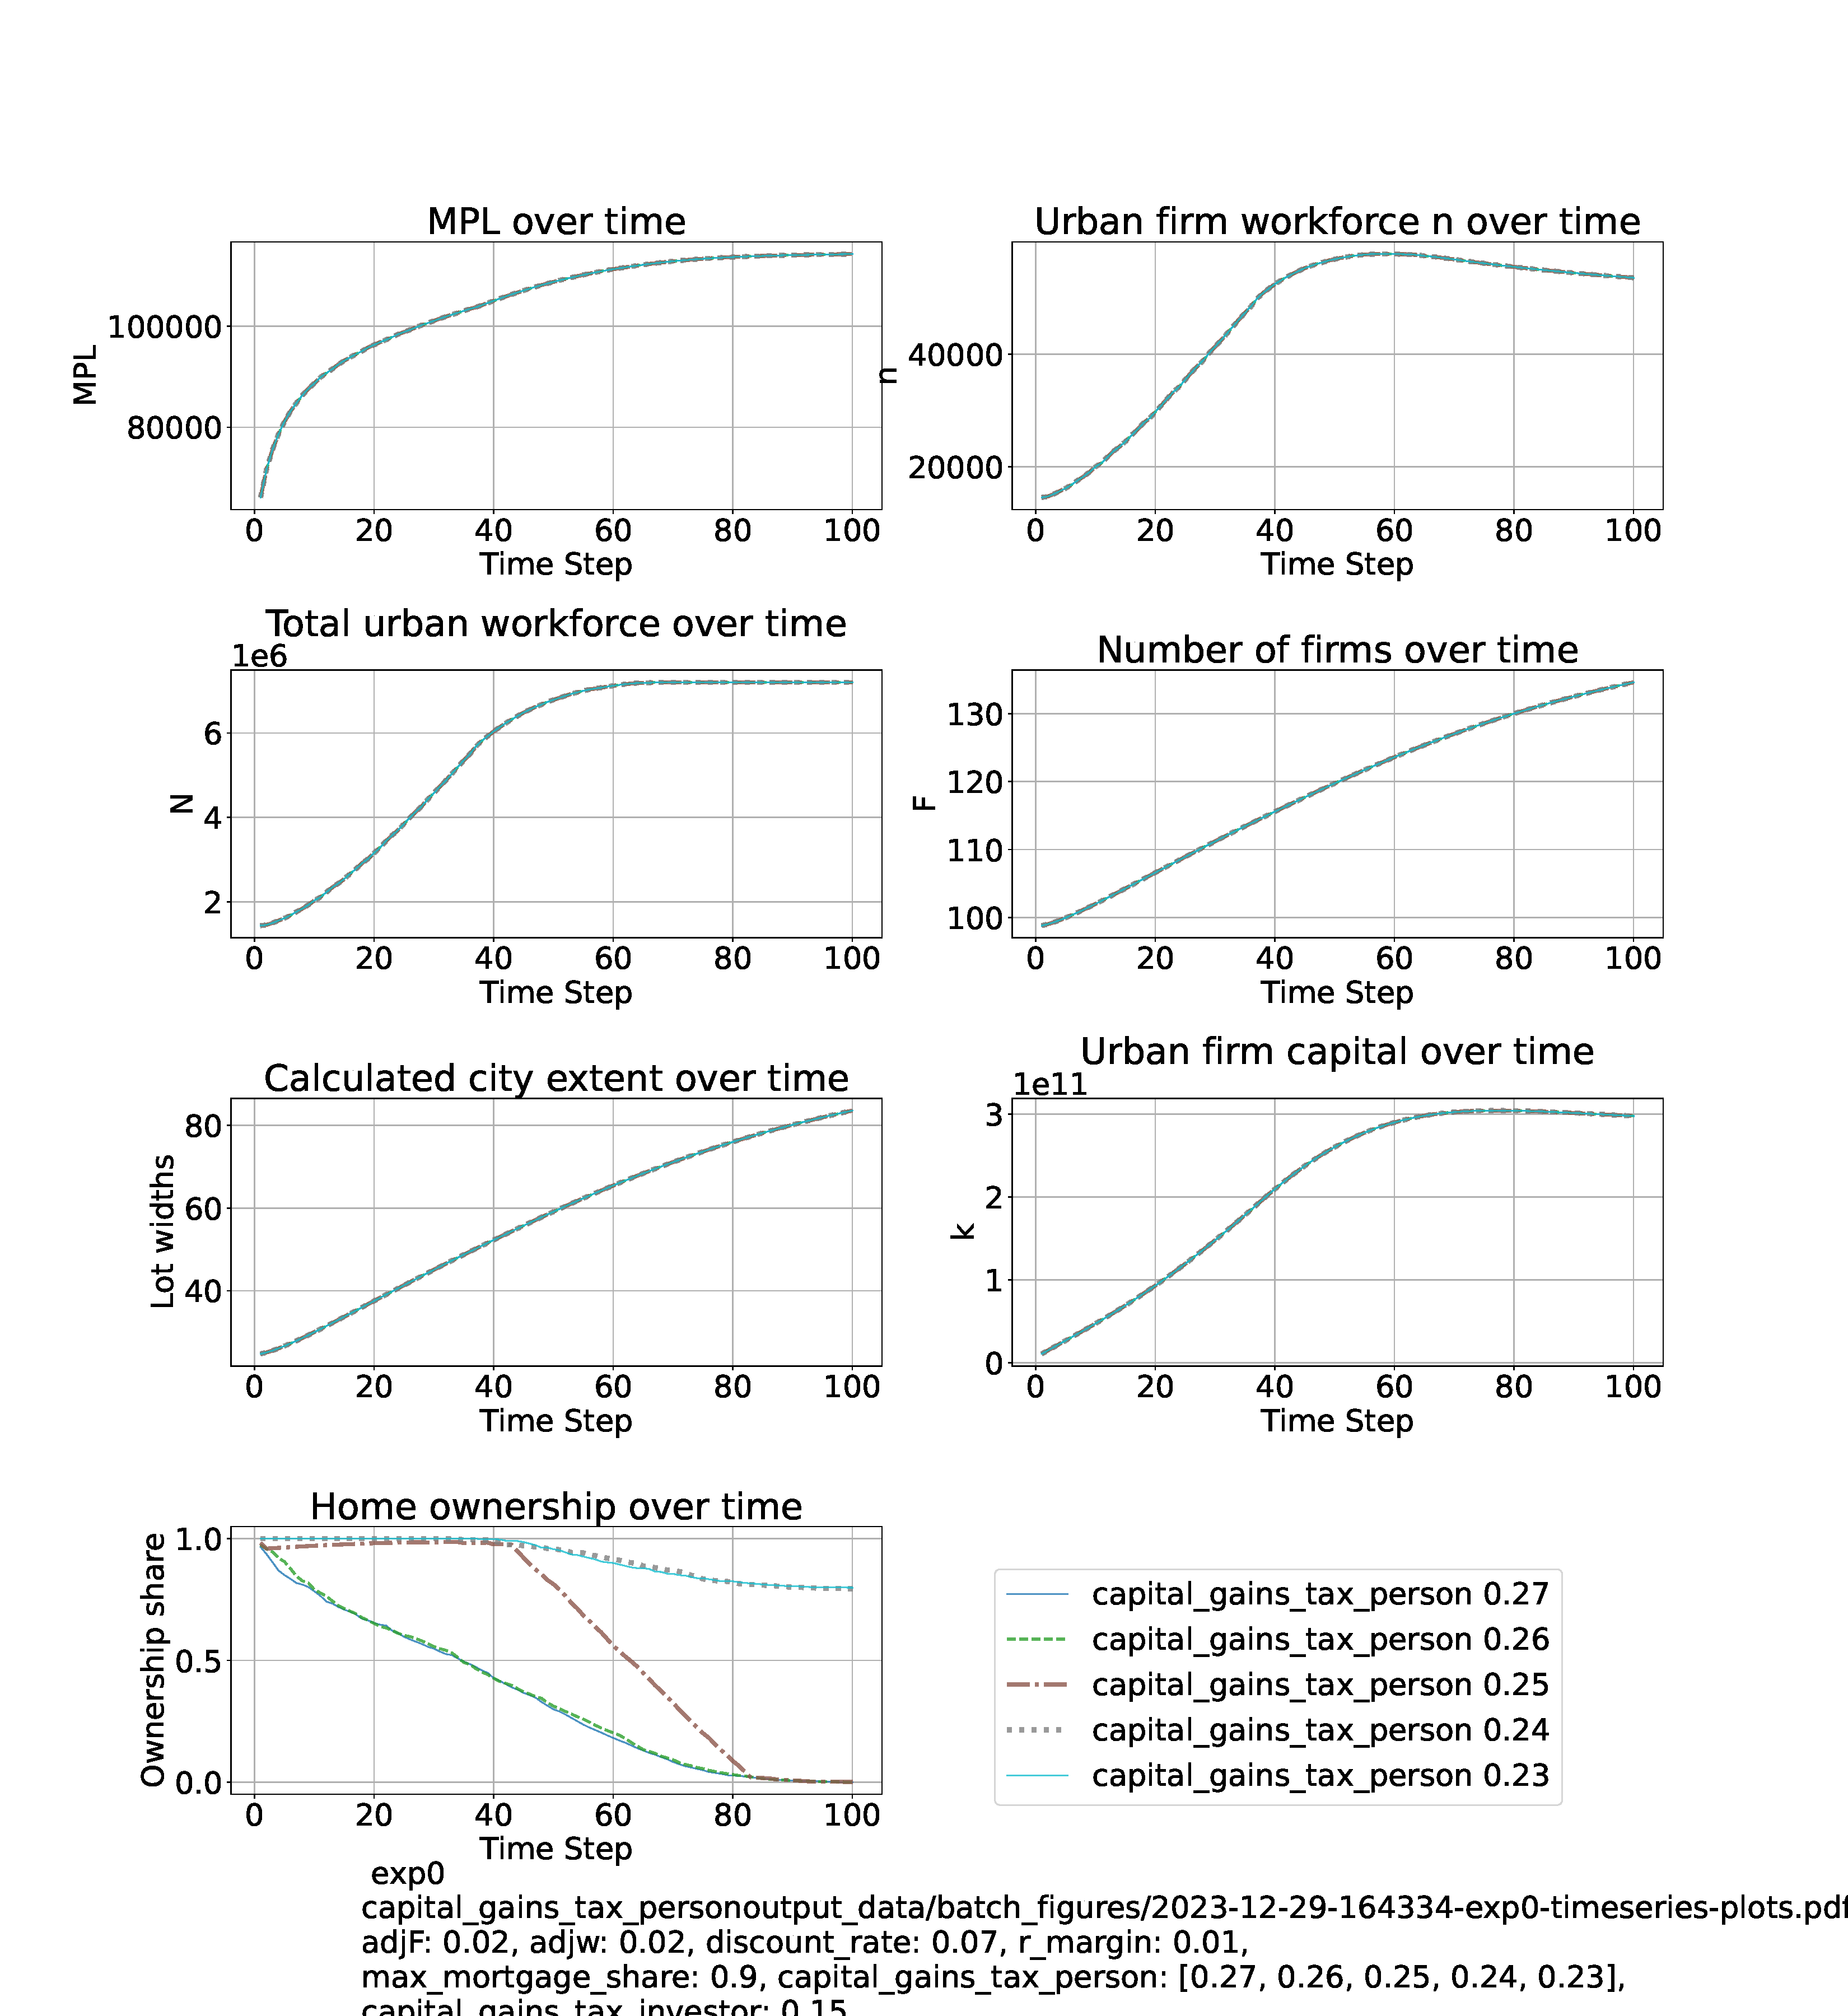
\includegraphics[trim= 1.5cm 3.65cm 2cm 4.0cm, clip, scale=.28]{fig/Analysis/Capital-gains-person-point27-6-5-4-3.pdf}


More precisely, we find that ownership stabilizes at 80\%  capital gains tax rates below 0.245. \textbf{(A gap is 0.1 in favour of households seems to be needed to support home-ownership.)}

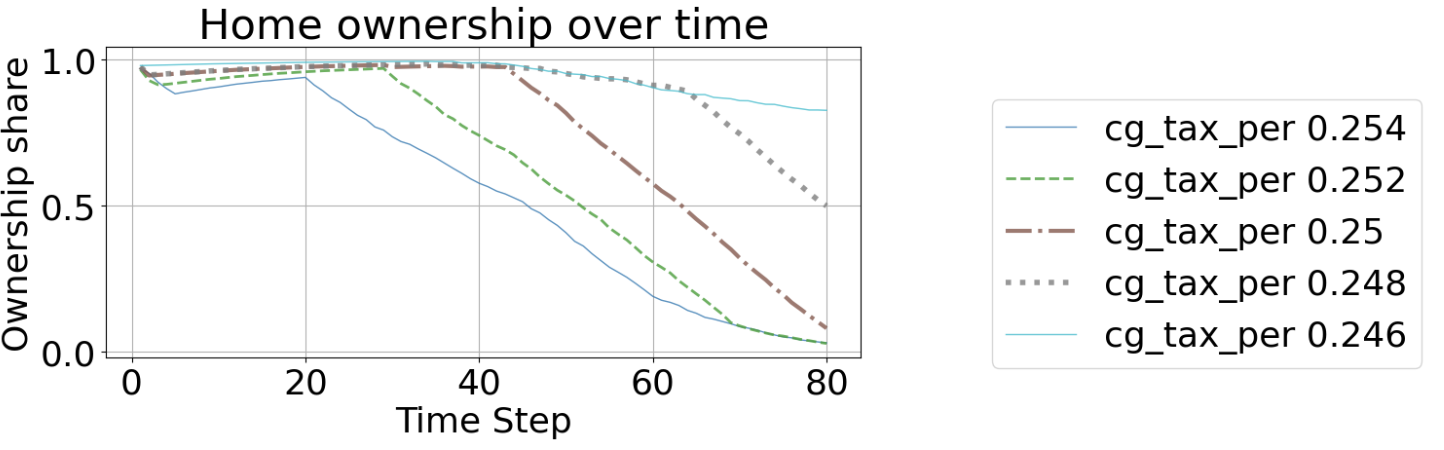
\includegraphics[ scale=.5]{fig/Analysis/Capital-gains-person-point246-254.png}


It should be possible to identify a boundary in the entire capital gains tax space between values of capital gains for investors and occupiers -owners where ownership begins to shift from occupiers to investors.

\vspace{1cm}
WORK IN PROGRESS

When the capital gains rate for \textbf{investors} is varied 

\newpage %%%%%%%%%%%%%%%%%%%%%%%%%%%%%%%%%%


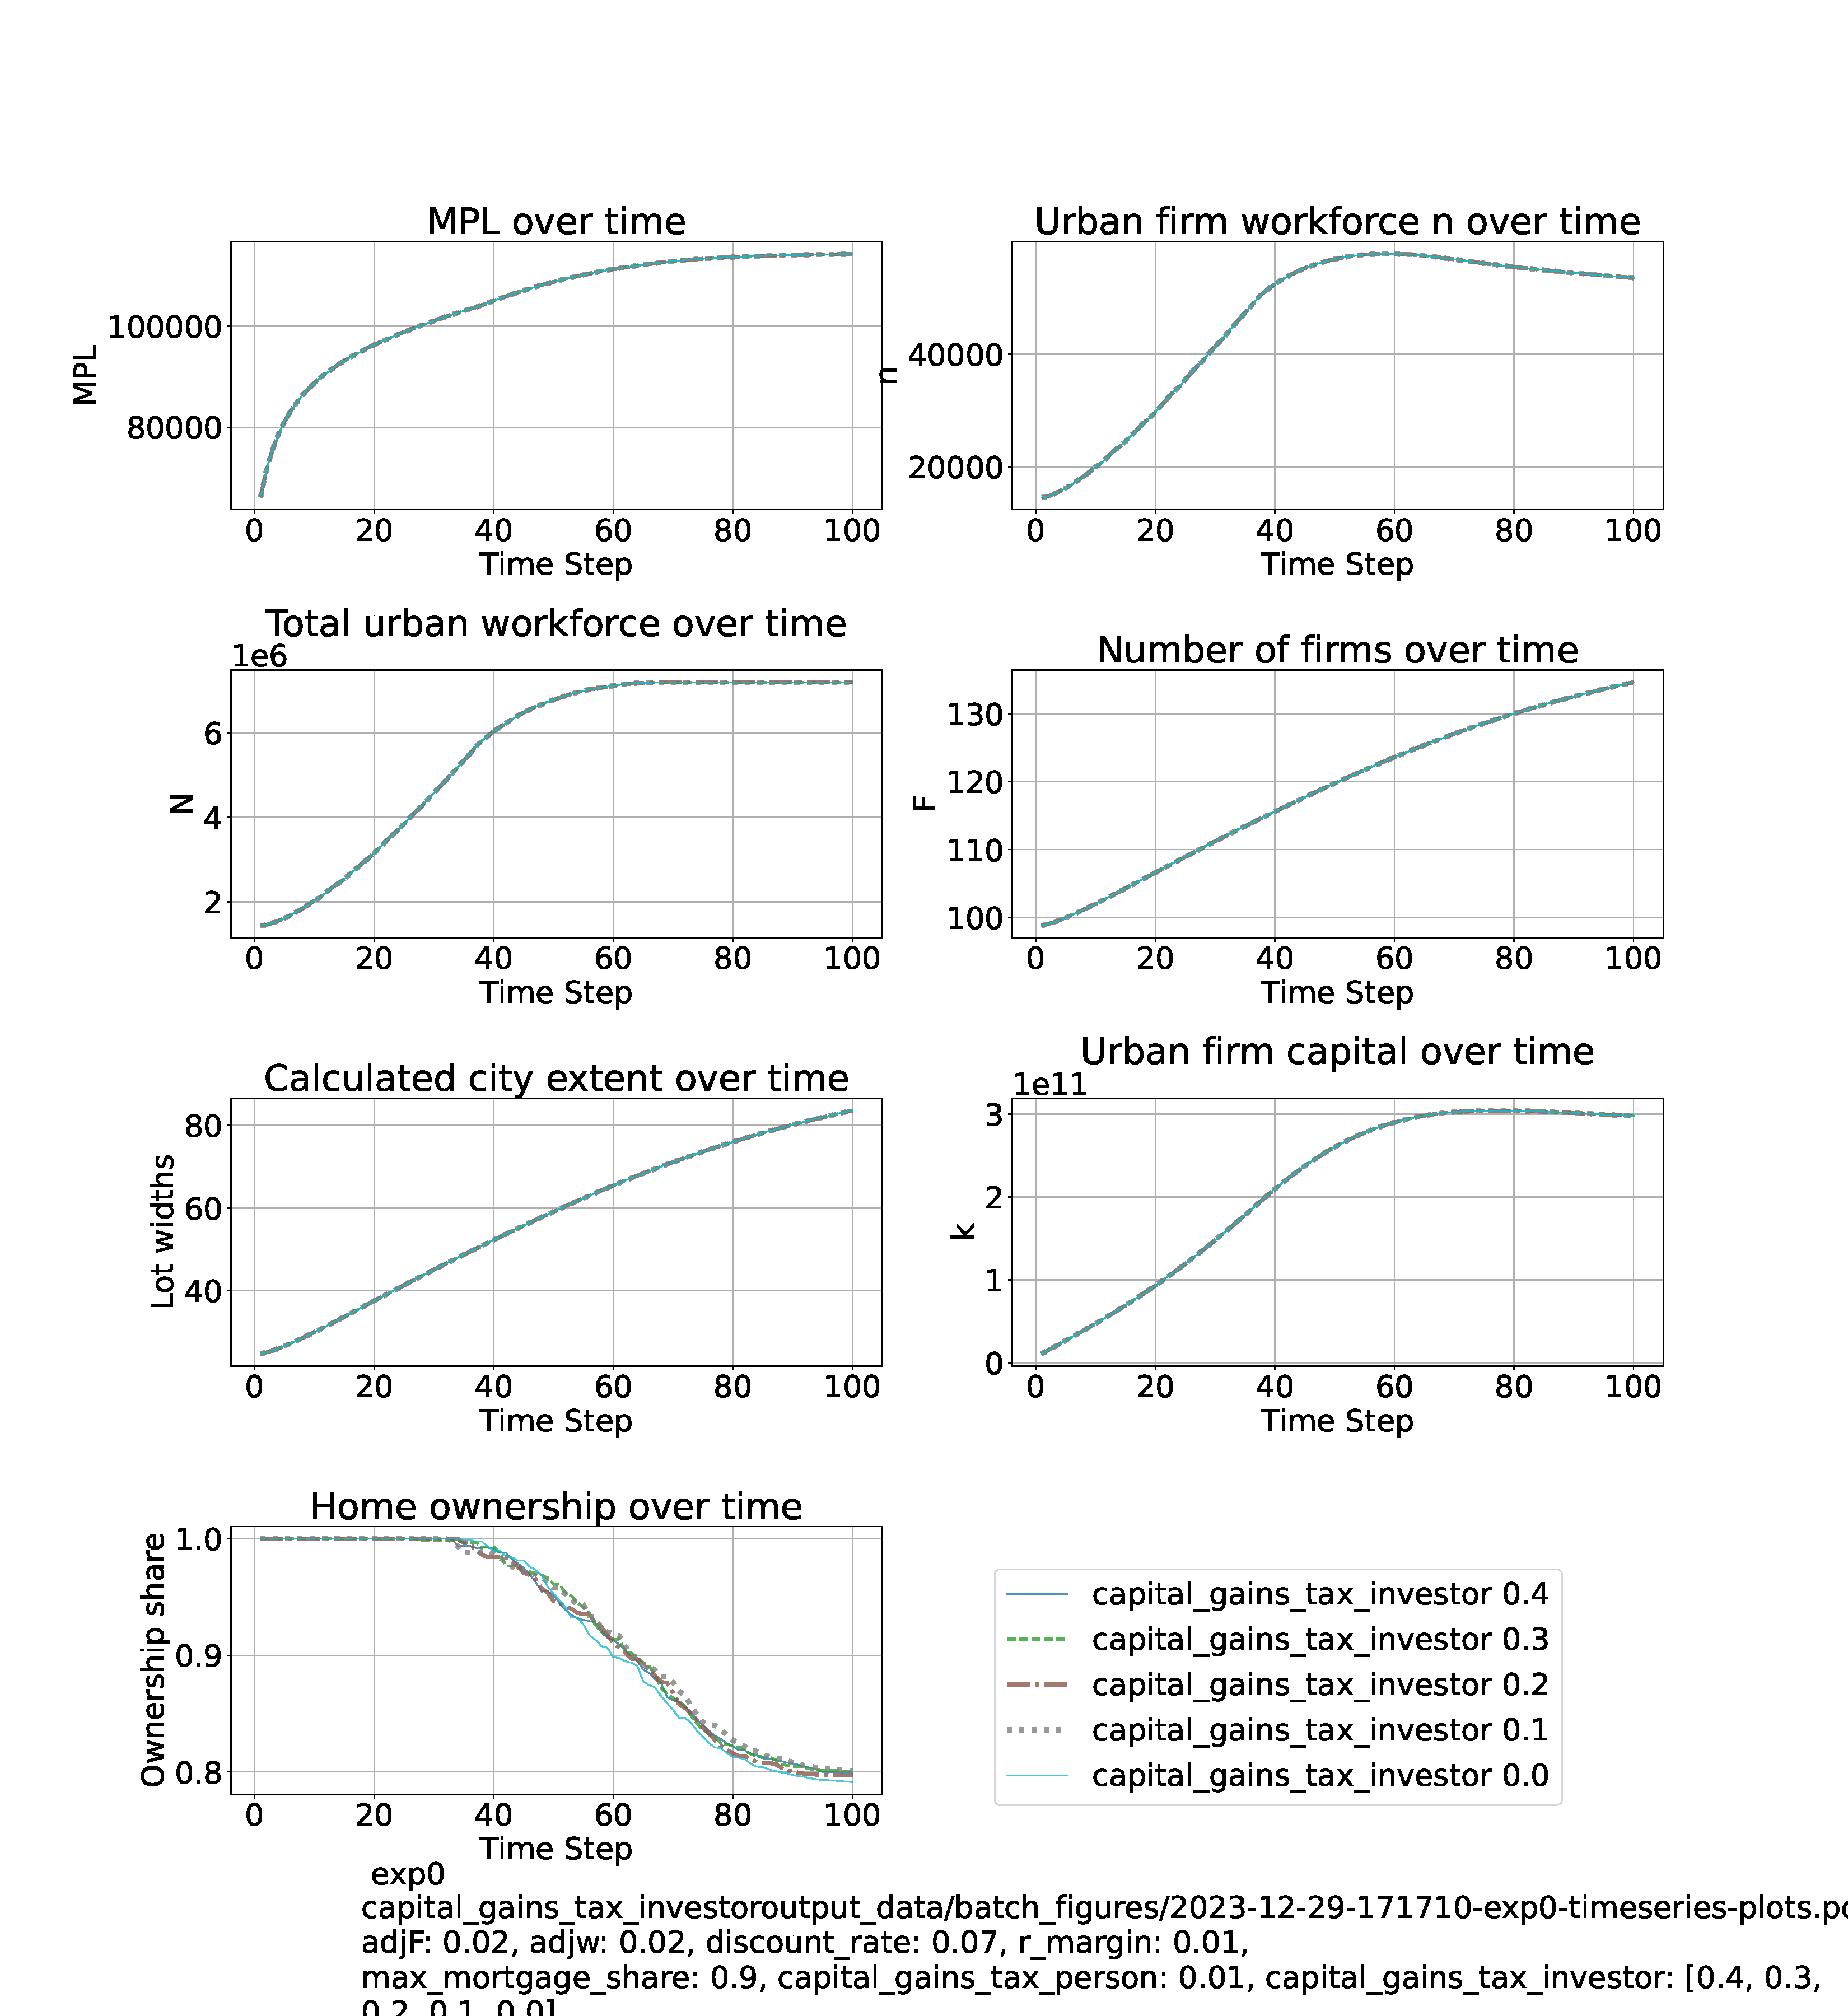
\includegraphics[trim= 1.5cm 3.65cm 2cm 4.0cm, clip, scale=.28]{fig/Analysis/Capital-gains-investor-point-4-3-2-1-0.pdf}



%%%%%%%%%%%%%%%%%%%%%%%%%%%%%%%%%%%%%%%%%%%%%
\newpage
\subsection{Working period}
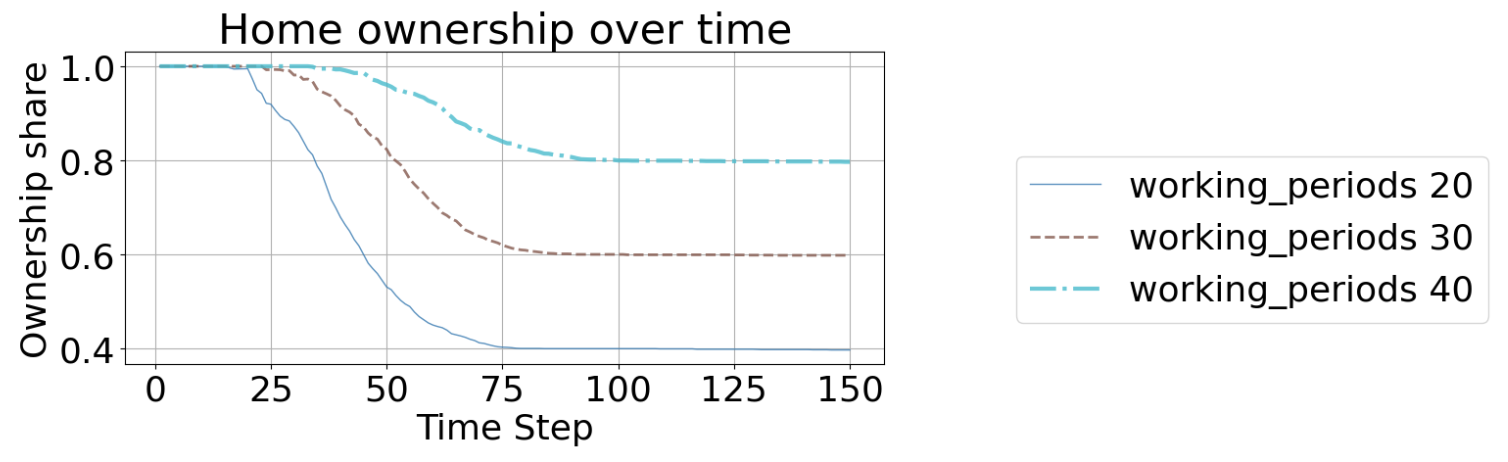
\includegraphics[ scale=.5]{fig/Analysis/Working-period 20-30-40.png}

The longer workers stay in the labour force the higher the fraction of the housing stock that is owner-occupied. this was an unexpected result. 

It is probably because when turnover is increased  institutional investors have m0re chances to get into the market. 

Savings for potential buyers are not obviously affected.

Shorter periods for owners to make capital gains may have an effect.

If the result reflects real processes, it is likely that increased workforce churn reduces owner-occupancy.





\subsection{Maximum Mortgage share}
Contrary to our expectations, the maximum fraction of a come that can be mortgaged appears not to affect  the base economic model and no effect on the pattern of ownership

\subsection{Income share used for mortgage}
This variable also has no effect. Combinations with Maximum Mortgage share have no effect.

%%%%%%%%%%%%%%%%%%%%%%%%%%%%%%%%%%
\newpage
\subsection{Property taxes}

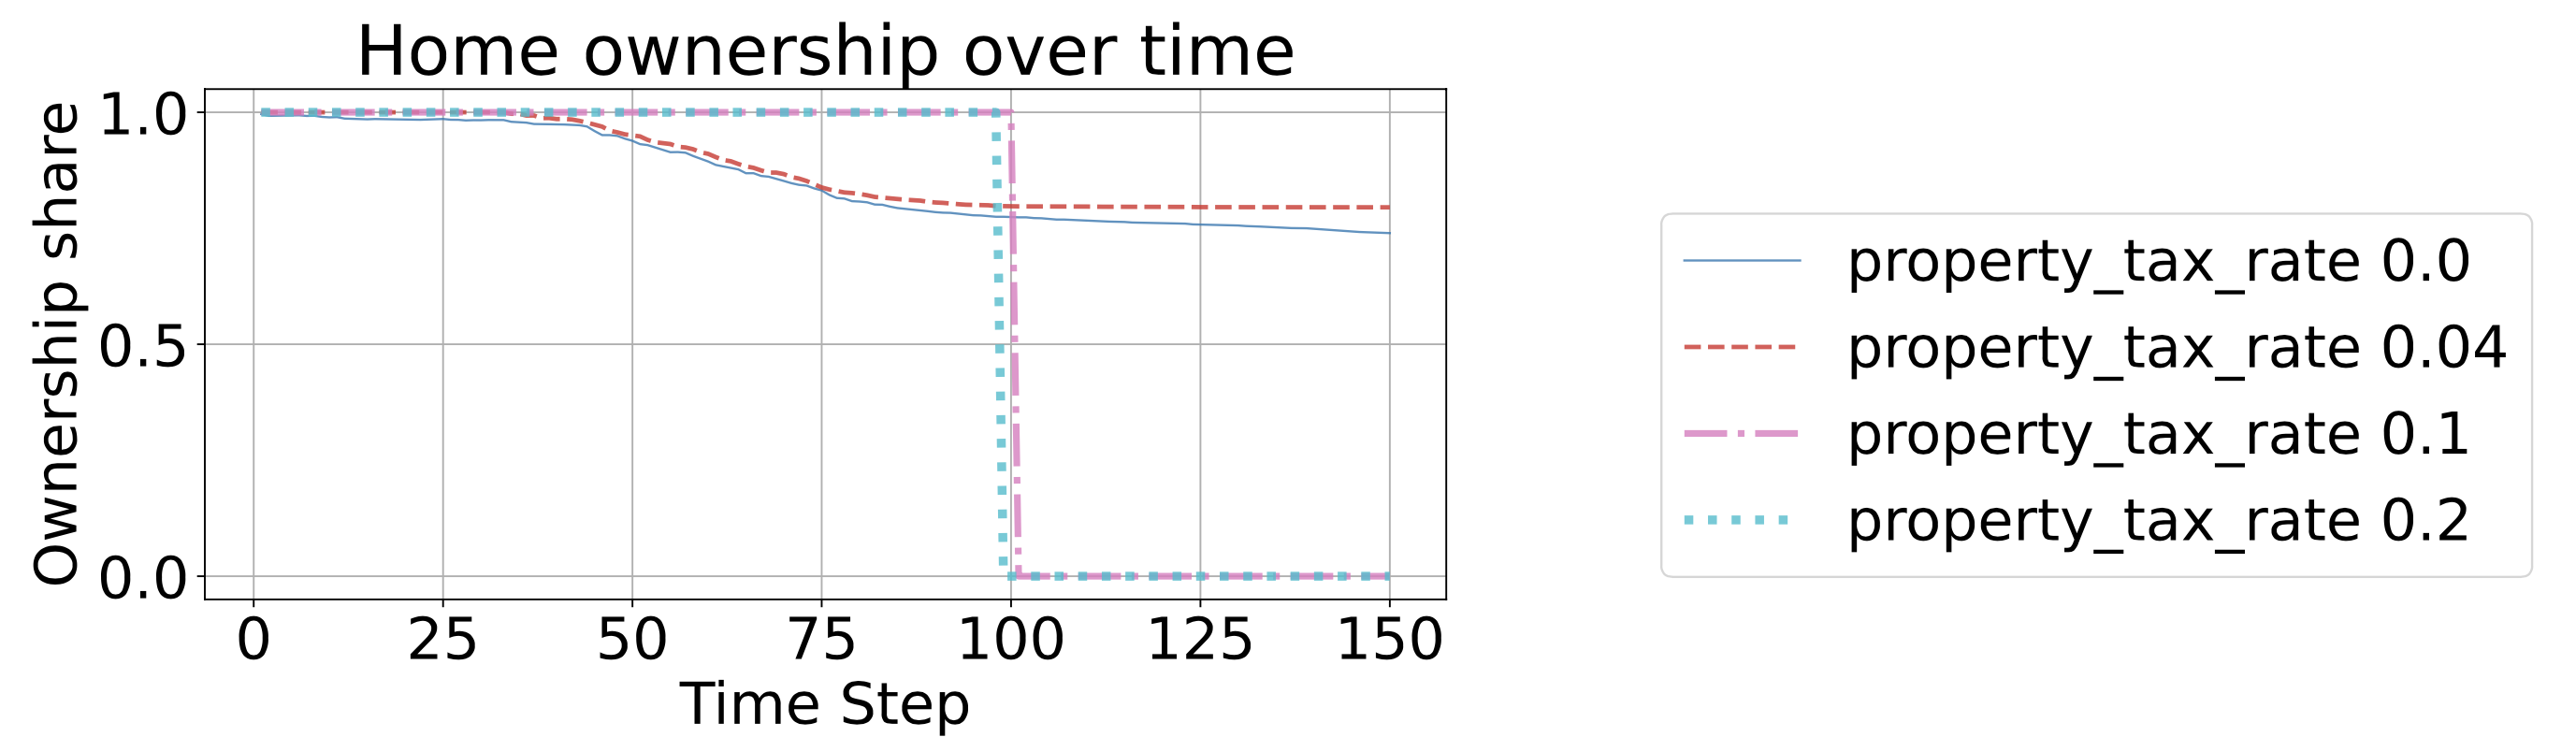
\includegraphics[ scale=.25]{fig/Analysis/Property-tax-point4-2.png}
At a property tax rate of 4.5\% we see a sharp change in the ownership pattern. Above this point owner-occupiers disappear. This seems reasonable, but the time pattern is strange. Why a sharp change at 100 time steps?

4\% approximates the level of actual mill-rates in Ontario.




% %%%%%%%%%%%%%%%%%%%%%%%%%%%%%%%%%%

% \subsection{Working period}

% 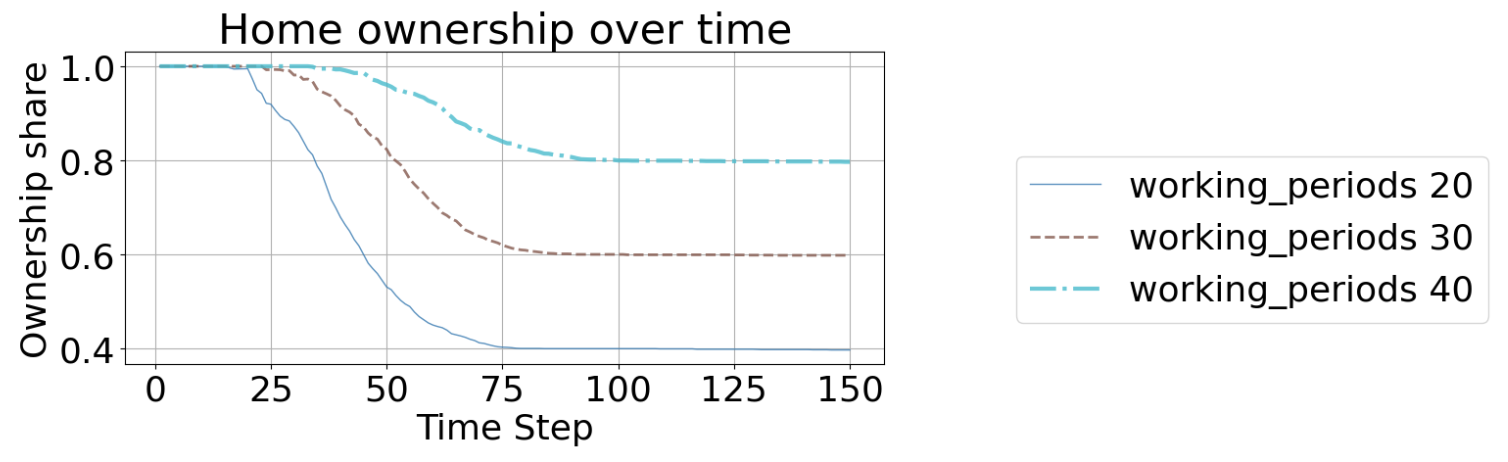
\includegraphics[ scale=.5]{fig/Analysis/Working-period 20-30-40.png}


%%%%%%%%%%%%%%%%%%%%%%%%%%%%%%%%%%
\subsection{12-15 -010050 Change wealth sensitivity two cases 0.1 and 0.05 }
no sensitivity in any output for this parameter base. Ownership share may show  a small effect if we are near a tipping point driven by p-dot

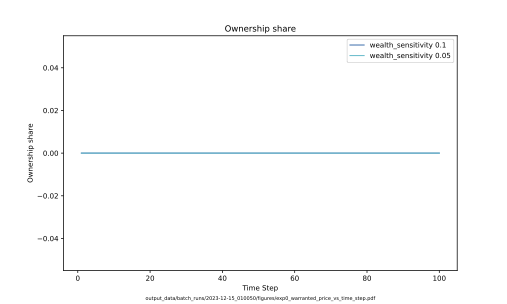
\includegraphics[scale=.45]{fig/Analysis/exp0_warranted_price_vs_time_step.png}


\begin{multicols}{2}
[\textbf{parameters}]
\begin{verbatim}
'adjn': 0.15,
'adjF': 0.02,
'adjw': 0.05, 
'capital_gains_tax_person':   0.0,
'capital_gains_tax_investor': 1,
\end{verbatim}

\end{multicols}


%%%%%%%%%%%%%%%%%%%%%%%%%%%%%%%%%%
\subsection{interest rate r-prime for investors}
Surprisingly we we no effect of doubling or halving r for investors.


%%%%%%%%%%%%%%%%%%%%%%%%%%%%%%%%%%
\subsection{Effect  of savings on bids}
Household savings produce the expected result: Below a critical level they prevent newcomers from bidding. in the interval from about \$30,000 to about100,00 bidders are wealth constrained. 

The Figures show a  three-dimensional surface as polygons. The significant details are  1) that the near-surface leans away, indicating bids rise as savings increase below \$100,00

and 2) the smallpatch in the nearest corner indicating no bids for the most distant properties from those with the least savings. this surprisede me because I would exp[ecxt no bids for the more expensive properties atr low savings]
 

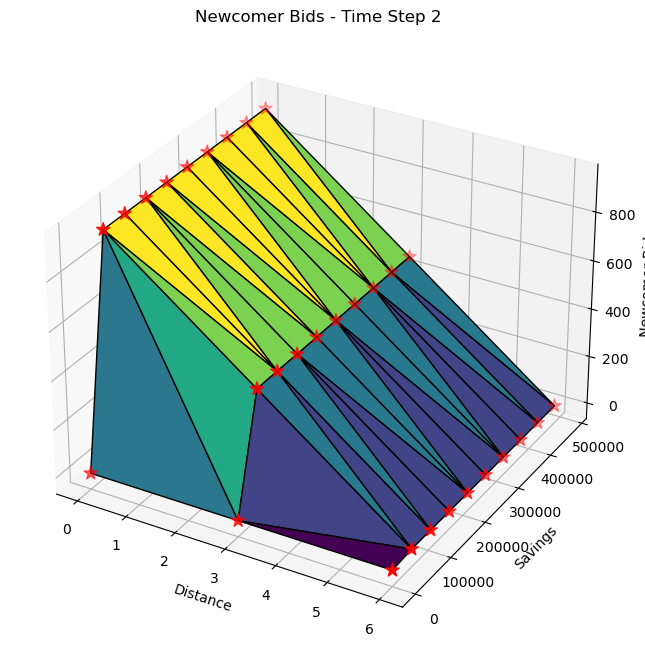
\includegraphics[scale=.9]{fig/Analysis/Savings-distanc-bids.png}



%%%%%%%%%%%%%%%%%%%%%%%%%%%%%%%%%%%%%%%%%%%%%

% %%%%%%%%%%%%%%%%%%%%%%%%%%%%%%%%%%%%%%%%%%%%
%  \subsection{12-17 010050, Varying Capital gains  }
% \begin{tabular}{c|c}
%   mpl  &  \\
%   n   &  \\
%   N   &  \\
%   F   &  \\
%   E   &  \\
%   k   & 
% \end{tabular} 

% \includegraphics[trim= 1.5cm 5cm 2cm 6.5cm, clip, scale=.40]{fig/Analysis/215330-exp0-timeseries-plots.pdf}

% adjF: 0.02, adjw: 0.15, discount_rate: 0.07, r_margin: 0.01, max_mortgage_share: 0.9,  capital_gains_tax_person: [0.5, 0.01], capital_gains_tax_investor: [0.75, 0.5, 0.25

% \includegraphics[scale=.4, trim=2cm  5cm 2cm 4cm, clip]{fig/Analysis/2023-12-17_215330_exp0_timeseries_plots.pdf}

 \end{document}

 \newpage
% \subsection{parameters}
% \begin{verbatim}

% \end{verbatim}

% \subsection{Change  12-15 010050}
\begin{tabular}{c|c}
  mpl  &  \\
  n   &  \\
  N   &  \\
  F   &  \\
  E   &  \\
  k   & 
\end{tabular} 

 \includegraphics[scale=.25]{215330-exp0-timeseries-plots.pdf}
